% 若编译失败,且生成 .synctex(busy) 辅助文件,可能有两个原因:
% 1. 需要插入的图片不存在:Ctrl + F 搜索 'figure' 将这些代码注释/删除掉即可
% 2. 路径/文件名含中文或空格:更改路径/文件名即可

% --------------------- 文章宏包及相关设置 --------------------- %
% >> ------------------ 文章宏包及相关设置 ------------------ << %
% 设定文章类型与编码格式
\documentclass[UTF8]{article}		

% 物理实验报告所需的其它宏包
\usepackage{ulem}   % \uline 下划线支持
\usepackage{circuitikz} % 电路图 tikz 支持
\usepackage{pdfpages}   % 用于导入 pdf 文件
\usepackage{multirow}   % 用于表格合并单元格

% 本 .tex 专属的宏定义
    \def\V{\ \mathrm{V}}
    \def\uV{\ \mu\mathrm{V}}
    \def\mV{\ \mathrm{mV}}
    \def\K{\ \mathrm{K}}
    \def\kV{\ \mathrm{KV}}
    \def\KV{\ \mathrm{KV}}
    \def\MV{\ \mathrm{MV}}
    \def\uA{\ \mu\mathrm{A}}
    \def\mA{\ \mathrm{mA}}
    \def\A{\ \mathrm{A}}
    \def\kA{\ \mathrm{KA}}
    \def\KA{\ \mathrm{KA}}
    \def\MA{\ \mathrm{MA}}
    \def\O{\ \Omega}
    \def\mO{\ \Omega}
    \def\kO{\ \mathrm{K}\Omega}
    \def\KO{\ \mathrm{K}\Omega}
    \def\MO{\ \mathrm{M}\Omega}
    \def\Hz{\ \mathrm{Hz}}
    \def\uF{\ \mu\mathrm{F}}
    \def\mF{\ \mathrm{mF}}
    \def\F{\ \mathrm{F}}
    \def\Re{\mathrm{\,Re}\,}
    \def\Im{\mathrm{\,Im}\,}
    \def\sinc{\mathrm{\,sinc}\,}

% 自定义宏定义
    \def\N{\mathbb{N}}
    \def\F{\mathbb{F}}
    \def\Z{\mathbb{Z}}
    \def\Q{\mathbb{Q}}
    \def\R{\mathbb{R}}
    \def\C{\mathbb{C}}
    \def\T{\mathbb{T}}
    \def\S{\mathbb{S}}
    %\def\A{\mathbb{A}}
    \def\I{\mathscr{I}}
    \def\d{\mathrm{d}}
    \def\p{\partial}


% 导入基本宏包
    \usepackage[UTF8]{ctex}     % 设置文档为中文语言
    \usepackage{hyperref}  % 宏包:自动生成超链接 (此宏包与标题中的数学环境冲突)
    \hypersetup{
        colorlinks=true,    % false:边框链接 ; true:彩色链接
        citecolor={blue},    % 文献引用颜色
        linkcolor={blue},   % 目录 (我们在目录处单独设置),公式,图表,脚注等内部链接颜色
        urlcolor={orange},    % 网页 URL 链接颜色,包括 \href 中的 text
        % cyan 浅蓝色 
        % magenta 洋红色
        % yellow 黄色
        % black 黑色
        % white 白色
        % red 红色
        % green 绿色
        % blue 蓝色
        % gray 灰色
        % darkgray 深灰色
        % lightgray 浅灰色
        % brown 棕色
        % lime 石灰色
        % olive 橄榄色
        % orange 橙色
        % pink 粉红色
        % purple 紫色
        % teal 蓝绿色
        % violet 紫罗兰色
    }
    % \usepackage{docmute}    % 宏包:子文件导入时自动去除导言区,用于主/子文件的写作方式,\include{./51单片机笔记}即可。注:启用此宏包会导致.tex文件capacity受限。
    \usepackage{amsmath}    % 宏包:数学公式
    \usepackage{mathrsfs}   % 宏包:提供更多数学符号
    \usepackage{amssymb}    % 宏包:提供更多数学符号
    \usepackage{pifont}     % 宏包:提供了特殊符号和字体
    \usepackage{extarrows}  % 宏包:更多箭头符号 
    \usepackage{multicol}   % 宏包:支持多栏 

% 文章页面margin设置
    \usepackage[a4paper]{geometry}
        \geometry{top=0.75in}
        \geometry{bottom=0.75in}
        \geometry{left=0.75in}
        \geometry{right=0.75in}   % 设置上下左右页边距
        \geometry{marginparwidth=1.75cm}    % 设置边注距离(注释、标记等)

% 配置数学环境
    \usepackage{amsthm} % 宏包:数学环境配置
    % theorem-line 环境自定义
        \newtheoremstyle{MyLineTheoremStyle}% <name>
            {11pt}% <space above>
            {11pt}% <space below>
            {}% <body font> 默认使用正文字体,  为楷体
            {}% <indent amount>
            {\bfseries}% <theorem head font> 设置标题项为加粗
            {:\ \ }% <punctuation after theorem head>
            {.5em}% <space after theorem head>
            {\textbf{#1}\thmnumber{#2}\ \ (\,\textbf{#3}\,)}% 设置标题内容顺序
        \theoremstyle{MyLineTheoremStyle} % 应用自定义的定理样式
        \newtheorem{LineTheorem}{Theorem.\,}
    % theorem-block 环境自定义
        \newtheoremstyle{MyBlockTheoremStyle}% <name>
            {11pt}% <space above>
            {11pt}% <space below>
            {}% <body font> 使用默认正文字体
            {}% <indent amount>
            {\bfseries}% <theorem head font> 设置标题项为加粗
            {:\\ \indent}% <punctuation after theorem head>
            {.5em}% <space after theorem head>
            {\textbf{#1}\thmnumber{#2}\ \ (\,\textbf{#3}\,)}% 设置标题内容顺序
        \theoremstyle{MyBlockTheoremStyle} % 应用自定义的定理样式
        \newtheorem{BlockTheorem}[LineTheorem]{Theorem.\,} % 使用 LineTheorem 的计数器
    % definition 环境自定义
        \newtheoremstyle{MySubsubsectionStyle}% <name>
            {11pt}% <space above>
            {11pt}% <space below>
            {}% <body font> 使用默认正文字体
            {}% <indent amount>
            {\bfseries}% <theorem head font> 设置标题项为加粗
            {:\\ \indent}% <punctuation after theorem head>
            {0pt}% <space after theorem head>
            {\textbf{#3}}% 设置标题内容顺序
        \theoremstyle{MySubsubsectionStyle} % 应用自定义的定理样式
        \newtheorem{definition}{}

%宏包:有色文本框(proof环境)及其设置
    \usepackage{xcolor}    %设置插入的文本框颜色
    \usepackage[strict]{changepage}     % 提供一个 adjustwidth 环境
    \usepackage{framed}     % 实现方框效果
        \definecolor{graybox_color}{rgb}{0.95,0.95,0.96} % 文本框颜色。修改此行中的 rgb 数值即可改变方框纹颜色,具体颜色的rgb数值可以在网站https://colordrop.io/ 中获得。(截止目前的尝试还没有成功过,感觉单位不一样)(找到喜欢的颜色,点击下方的小眼睛,找到rgb值,复制修改即可)
        \newenvironment{graybox}{%
        \def\FrameCommand{%
        \hspace{1pt}%
        {\color{gray}\vrule width 2pt}%
        {\color{graybox_color}\vrule width 4pt}%
        \colorbox{graybox_color}%
        }%
        \MakeFramed{\advance\hsize-\width\FrameRestore}%
        \noindent\hspace{-4.55pt}% disable indenting first paragraph
        \begin{adjustwidth}{}{7pt}%
        \vspace{2pt}\vspace{2pt}%
        }
        {%
        \vspace{2pt}\end{adjustwidth}\endMakeFramed%
        }

% 外源代码插入设置
    % matlab 代码插入设置
    \usepackage{matlab-prettifier}
        \lstset{style=Matlab-editor}    % 继承 matlab 代码高亮 , 此行不能删去
    \usepackage[most]{tcolorbox} % 引入tcolorbox包 
    \usepackage{listings} % 引入listings包
        \tcbuselibrary{listings, skins, breakable}
        \newfontfamily\codefont{Consolas} % 定义需要的 codefont 字体
        \lstdefinestyle{MatlabStyle_inc}{   % 插入代码的样式
            language=Matlab,
            basicstyle=\footnotesize\ttfamily\codefont,    % ttfamily 确保等宽 
            breakatwhitespace=false,
            breaklines=true,
            captionpos=b,
            keepspaces=true,
            numbers=left,
            numbersep=15pt,
            showspaces=false,
            showstringspaces=false,
            showtabs=false,
            tabsize=2,
            xleftmargin=15pt,   % 左边距
            %frame=single, % single 为包围式单线框
            frame=shadowbox,    % shadowbox 为带阴影包围式单线框效果
            %escapeinside=``,   % 允许在代码块中使用 LaTeX 命令 (此行无用)
            %frameround=tttt,    % tttt 表示四个角都是圆角
            framextopmargin=0pt,    % 边框上边距
            framexbottommargin=0pt, % 边框下边距
            framexleftmargin=5pt,   % 边框左边距
            framexrightmargin=5pt,  % 边框右边距
            rulesepcolor=\color{red!20!green!20!blue!20}, % 阴影框颜色设置
            %backgroundcolor=\color{blue!10}, % 背景颜色
        }
        \lstdefinestyle{MatlabStyle_src}{   % 插入代码的样式
            language=Matlab,
            basicstyle=\small\ttfamily\codefont,    % ttfamily 确保等宽 
            breakatwhitespace=false,
            breaklines=true,
            captionpos=b,
            keepspaces=true,
            numbers=left,
            numbersep=15pt,
            showspaces=false,
            showstringspaces=false,
            showtabs=false,
            tabsize=2,
        }
        \newtcblisting{matlablisting}{
            %arc=2pt,        % 圆角半径
            % 调整代码在 listing 中的位置以和引入文件时的格式相同
            top=0pt,
            bottom=0pt,
            left=-5pt,
            right=-5pt,
            listing only,   % 此句不能删去
            listing style=MatlabStyle_src,
            breakable,
            colback=white,   % 选一个合适的颜色
            colframe=black!0,   % 感叹号后跟不透明度 (为 0 时完全透明)
        }
        \lstset{
            style=MatlabStyle_inc,
        }

% table 支持
    \usepackage{booktabs}   % 宏包:三线表
    \usepackage{tabularray} % 宏包:表格排版
    \usepackage{longtable}  % 宏包:长表格

% figure 设置
    \usepackage{graphicx}  % 支持 jpg, png, eps, pdf 图片 
    \usepackage{svg}       % 支持 svg 图片
        \svgsetup{
            % 指向 inkscape.exe 的路径
            inkscapeexe = C:/aa_MySame/inkscape/bin/inkscape.exe, 
            % 一定程度上修复导入后图片文字溢出几何图形的问题
            inkscapelatex = false                 
        }
    \usepackage{subcaption} % 用于子图和小图注  

% 图表进阶设置
    \usepackage{caption}    % 图注、表注
        \captionsetup[figure]{name=图}  
        \captionsetup[table]{name=表}
        \captionsetup{
            labelfont=bf, % 设置标签为粗体
            textfont=bf,  % 设置文本为粗体
            font=small  
        }
    \usepackage{float}     % 图表位置浮动设置 
    \usepackage{etoolbox} % 用于保证图注表注的数学字符为粗体
        \AtBeginEnvironment{figure}{\boldmath} % 图注中的数学字符为粗体
        \AtBeginEnvironment{table}{\boldmath}  % 表注中的数学字符为粗体
        \AtBeginEnvironment{tabular}{\unboldmath}   % 保证表格中的数学字符不受额外影响

% 圆圈序号自定义
    \newcommand*\circled[1]{\tikz[baseline=(char.base)]{\node[shape=circle,draw,inner sep=0.8pt, line width = 0.03em] (char) {\bfseries #1};}}   % TikZ solution

% 列表设置
    \usepackage{enumitem}   % 宏包:列表环境设置
        \setlist[enumerate]{
            label=(\arabic*) ,   % 设置序号样式为加粗的 (1) (2) (3)
            ref=\arabic*, % 如果需要引用列表项,这将决定引用格式(这里仍然使用数字)
            itemsep=0pt, parsep=0pt, topsep=0pt, partopsep=0pt, leftmargin=3.5em} 
        \setlist[itemize]{itemsep=0pt, parsep=0pt, topsep=0pt, partopsep=0pt, leftmargin=3.5em}
        \newlist{circledenum}{enumerate}{1} % 创建一个新的枚举环境  
        \setlist[circledenum,1]{  
            label=\protect\circled{\arabic*}, % 使用 \arabic* 来获取当前枚举计数器的值,并用 \circled 包装它  
            ref=\arabic*, % 如果需要引用列表项,这将决定引用格式(这里仍然使用数字)
            itemsep=0pt, parsep=0pt, topsep=0pt, partopsep=0pt, leftmargin=3.5em
        }  

% 其它设置
    % 脚注设置
        \renewcommand\thefootnote{\ding{\numexpr171+\value{footnote}}}
    % 参考文献引用设置
        \bibliographystyle{unsrt}   % 设置参考文献引用格式为unsrt
        \newcommand{\upcite}[1]{\textsuperscript{\cite{#1}}}     % 自定义上角标式引用
    % 文章序言设置
        \newcommand{\cnabstractname}{序言}
        \newenvironment{cnabstract}{%
            \par\Large
            \noindent\mbox{}\hfill{\bfseries \cnabstractname}\hfill\mbox{}\par
            \vskip 2.5ex
            }{\par\vskip 2.5ex}

% 文章默认字体设置
    \usepackage{fontspec}   % 宏包:字体设置
        \setmainfont{SimSun}    % 设置中文字体为宋体字体
        \setCJKmainfont[AutoFakeBold=3]{SimSun} % 设置加粗字体为 SimSun 族,AutoFakeBold 可以调整字体粗细
        \setmainfont{Times New Roman} % 设置英文字体为Times New Roman

% 各级标题自定义设置
    \usepackage{titlesec}   
        % section标题自定义设置 
        \titleformat{\section}[hang]{\normalfont\Large\bfseries\boldmath}{\thesection}{8pt}{}
        % subsection 标题自定义设置
        \titleformat{\subsection}[hang]{\normalfont\large\bfseries\boldmath}{\thesubsection}{8pt}{}
        \titlespacing*{\subsection}{0pt}{10pt}{6pt} % 控制上下间距


% --------------------- 文章宏包及相关设置 --------------------- %
% >> ------------------ 文章宏包及相关设置 ------------------ << %


% ------------------------ 文章信息区 ------------------------ %
% ------------------------ 文章信息区 ------------------------ %

% 每次实验报告需要修改的信息有:
% 1. 左上角页眉  
% 2. 实验名称  
% 3. 实验日期  
% 4. 实验地点  
% 5. 指导教师  

% 页眉页脚设置
\usepackage{fancyhdr}   %宏包:页眉页脚设置
    \pagestyle{fancy}
    \fancyhf{}
    \cfoot{\thepage}
    \renewcommand\headrulewidth{1pt}
    \renewcommand\footrulewidth{0pt}
    \rhead{\bfseries \large {\color{red} 分组序号: 2-05}}
    \chead{《基础物理实验》实验报告,\ 丁毅,\ 2023K8009908031}
    \lhead{\small Ex.05 气垫导轨 (2024.12.17)}
\begin{document}


\begin{center}\large
    \vspace*{-0.6cm}
    \noindent{\huge\bfseries《\ \ 基\ \ 础\ \ 物\ \ 理\ \ 实\ \ 验\ \ \ 》\ \ 实\ \ 验\ \ 报\ \ 告 }
    \\\vspace{0.3cm}
    \noindent{
    {\bfseries 
    实验名称:\uline{\hspace{0.cm} 气轨弹簧振子的简谐振动 \hspace{0.cm}}
    }\hspace{0.2cm}
    指导教师:\uline{\hspace{0.cm}余运林晨 \  \ yuyunlinchen21@mails.ucas.ac.cn \hspace{0.cm}}
    }
    \\\vspace{0.1cm}
    \noindent
    {
    姓名:\uline{\,\,\,丁毅\,\,\,}\hspace{0.2cm}
    学号:\uline{\,\,\,{ 2023K8009908031}\,\,\,}\hspace{0.2cm}
    班级/专业:\uline{\,\,\,{2308/电子信息}\,\,\,}\hspace{0.2cm}
    分组序号:\uline{\,\,\,{2-05}\,\,\,}
    }
    \\\vspace{0.1cm}
    \noindent{
    实验日期:\uline{\,\,{ 2024.12.17}\,\,}\hspace{0.2cm}
    实验地点:\uline{\,\,\,教学楼{716}\,\,\,}\hspace{0.2cm}
    是否调课/补课:\uline{\hspace{0.26cm}否 \hspace{0.26cm}}\hspace{0.2cm}
    成绩:\uline{\hspace{2cm}}
    }
\end{center}
\vspace{-0.3cm}
\noindent\rule{\textwidth}{0.075em}   % 分割线
\vspace{-1.1cm}

% 目录
%\zihao{-5}
\setcounter{tocdepth}{3}  % 目录深度为 2(不显示 subsubsection)
\noindent\tableofcontents\thispagestyle{fancy}   % 显示页码、页眉等
\newpage
\rhead{\bfseries\small 分组序号: 2-05}
\zihao{5}
% ------------------------ 文章信息区 ------------------------ %
% ------------------------ 文章信息区 ------------------------ %


%% 下面是正文内容


\section{实验目的}
\begin{enumerate}
    \item 观察简谐振动现象,测定简谐振动的周期。
    \item 求弹簧的倔强系数$k$和有效质量$m_0$。
    \item 观察简谐振动的运动学特征。
    \item 验证机械能守恒定律。
    \item 用极限法测定瞬时速度。
    \item 深入了解平均速度和瞬时速度的关系。
\end{enumerate}

\section{实验仪器}
    气垫导轨、滑块、附加砝码、弹簧、 U 型挡光片、平板挡光片、数字毫秒计、天平等。

\section{实验原理}
\subsection{弹簧振子的间谐运动}
在水平的气垫导轨上,两个相同的弹簧中间系一个滑块,滑块做往返振动,
若不考虑滑块运动的阻力,可以认为滑块的振动是理想的简谐振动。

设质量为$m_1$的滑块初始时处于平衡位置,此时每个弹簧的初始伸长量为$x_0$,当滑块偏离平衡点x
时,受弹性力$-k_1(x+x_0)$与$-k_1(x-x_0)$的作用,其中$k_1$是弹簧的倔强系数。根据牛顿第二定律,列出其运
动方程:$ - kx = m\ddot x$,其中 $k = 2 k_1$。

式中的 $m$与弹簧质量$m_1$并不相同。因为事实上弹簧也是有一定质量的,这导致了实际的运动并非严
格的简谐振动,而是需要考虑弹簧内部形成的驻波,详细推导需要采用分离变量法解微分方程,这里直接
给出结果:若在近似的仍欲采用简谐振动的结论,则可考虑只取一级近似,引入“弹簧有效质量”$m_0$

由一级近似可计算得$m = m_1 + m_0$,$m_0$为弹簧质量的$\frac{1}{3}$,这样对应该方程的解为:
\begin{equation}
    x = A\sin ({\omega _0}t + {\varphi _0})\quad {\omega _0} = \sqrt {\frac{k}{m}} 
\end{equation}

其中周期与固有频率的关系为
\begin{equation}
    T = \frac{{2\pi }}{{{\omega _0}}} = 2\pi \sqrt {\frac{m}{k}}  = 2\pi \sqrt {\frac{{{m_1} + {m_0}}}{k}} 
\end{equation}

将上式两边平方可以得到
\begin{equation}
    {T^2} = \frac{{4{\pi ^2}\left( {{m_1} + {m_0}} \right)}}{k}
\end{equation}

在实验中,我们改变$m_1$,测出相应的$T$,采用作图法获得$T-m_1$的曲线,理论上该曲线应为一条直
线,直线的斜率为$\frac{4 \pi^2}{k}$,采用最小二乘法可以计算出该直线的斜率,进而算出劲度系数到$k$的值。同
时,可以从该条直线的截距获取$m_0$的值。也可采用逐差法求解k和$m_0$的值。

\subsection{简谐运动的运动学特征}
运动方程两边同时对时间求导,即可得到
\begin{equation}
    v = \frac{{dx}}{{dt}} = A{\omega _0}\cos \left( {{\omega _0}t + {\varphi _0}} \right)
\end{equation}

由此可见,速度v与时间有关,且随时间的变化关系也为简谐振动,角频率为$\omega_0$,振幅为$A \omega_0$,而且
度$v$的相位比位移$x$超前$\frac{\pi}{2}$

联立$x$-$t$方程与$v$-$t$方程,消去时间$t$,即可得到
\begin{equation}
    {v^2} = \omega _0^2\left( {{A^2} - {x^2}} \right)
\end{equation}

当$x=A$时,$v=0$;当$x=0$时,$v =  \pm A{\omega _0}$,此时$v$取最大值

本实验可以通过观察$x$和$v$随时间的变化规律,以及$x$和$v$之间的相位关系。利用拟合的方法算出角频
率。

\subsection{简谐振动的机械能}
在实验中,任何时刻系统的振动动能为
\begin{equation}
    {E_k} = \frac{1}{2}m{v^2} = \frac{1}{2}\left( {{m_1} + {m_2}} \right){v^2}
\end{equation}

由于此前在第一个实验项目中,已经测得弹簧的劲度系数为$k$,因此可以直接算得系统的弹性势能为
(以$m_1$位于平衡位置时系统的势能为零)

\begin{equation}
    {E_p} = \frac{1}{2}k{x^2}
\end{equation}

所以系统的机械能为
\begin{equation}
    E = {E_k} + {E_p} = \frac{1}{2}m{\omega ^2}{A^2} = \frac{1}{2}k{A^2}
\end{equation}

上式中的$k$和$A$均不随时间变化

通过测量滑块$m_1$在不同位置$x$的速度$v$,从而计算弹性势能和振动势能,并验证他们之间的相互转换
关系和机械能守恒定律是否吻合。

\subsection{瞬时速度的测量}
设变速运动的物体在 $\Delta t$ 时间中经过的路程为$\Delta s$,则其平均速度为$\overline v  = \frac{{\Delta s}}{{\Delta t}}$

当$\Delta t$与$\Delta s$均趋于0时,平均速度的极限就为物体的瞬时速度。

在实验中,在倾斜的气轨上,于A点处放置一光电门,在滑块上先后安装上挡光距离不同的U形
挡光片,使各挡光片的第一挡光边距A点为l。滑块每次自P点由静止开始下滑,分别测出相应的挡光
时间$\Delta t$及挡光距离$\Delta s$。(设滑块由静止下滑距离l后的瞬时速度为$v_0$即第一挡光时滑块的瞬时速度),
则有:
\begin{equation}
    \overline v  = \frac{{\Delta s}}{{\Delta t}} = {v_0} + \frac{1}{2}a \cdot \Delta t
\end{equation}

其中$a$为物体在A点附近的加速度
本实验可以通过改变挡光距离$\Delta s$观察平均速度和瞬时速度的关系,分别画出 $v$-$t$ 图和 $v$-$x$ 图,利用外
推法求出瞬时速度。

\section{实验内容}

\begin{enumerate}
\item 学会光电门测速和测周期的使用方法。
\item 调节气垫导轨至水平状态,通过测量任意两点的速度变化,验证气垫导轨是否处于
水平状态。
\item 测量弹簧振子的振动周期并考察振动周期和振幅的关系。滑块的振幅 A 分别取
10.0、 20.0、 30.0、 40.0 cm 时,测量其相应振动周期。分析和讨论实验结果可得出什么
结论? 
\item 研究振动周期和振子质量之间的关系。在滑块上加骑码(铁片)。对一个确定的振幅
(如取 A=40.0 cm)每增加一个骑码测量一组周期 $T$。(骑码不能加太多,以阻尼不明显为限。) 
作 $T^2$-$m$ 的图,如果 $T$与 $m$ 的关系式如公式所示,则$T^2$-$m$ 的图应为一条直线,
其斜率为 $4$$\pi^2$/$k$,截距为$4$$\pi^2$$m_0$/$k$ 。用最小二乘法做直线拟合,求出 $k$ 和 $m_0$。
\item 研究速度和位移的关系。在滑块上装上 U 型挡光片,可测量速度。
作 $v^2$-$x^2$的图,看该图是否为一条直线,并进行直线拟合,看斜率是否为 $-\omega_0^2$ ,截
距是否为 $A^2$$\omega_0^2$,其中$\omega_0=2\pi /T $ ,$T$ 可测出。
\item 研究振动系统的机械能是否守恒。固定振幅(如取 A=40.0 cm),测出不同$x$处的滑
块速度,由此算出振动过程中经过每一个$x$处的动能和势能,并对各$x$处的机械能进行比
较,得出结论。
\item 研究平均速度与瞬时速度的关系,利用外推法求出瞬时速度。在气轨下面只有一个螺丝的一端,小心将气轨抬起来,把垫块放到这个螺丝的下面。测量具有不同$\Delta s$的挡光片在
距离 A 点为 50cm 处从静止开始自由下滑,从 A 点开始在$\Delta s$所用的时间$\Delta t$,求出平均速度$\overline{v}$ ,作$\overline{v}-\Delta t$图和$\overline{v}-\Delta s $图,将图线性外推求出瞬时速度$v_0$。
\item 通过改变气轨的倾斜角度$\theta $(增加垫块数量),重复上述实验。
\item 通过改变 A 点到 P 点的距离 $l$(设置 60 cm 处),重复上述实验。

\end{enumerate}


\section{实验数据及数据处理}

\subsection{实验仪器调试}
调试结果如下表所示,其中 $\eta = \frac{v_2 - v_1}{v_1} \times 100 \,\%$。
\begin{table}[H]\centering
    %\renewcommand{\arraystretch}{1.5} % 调整行间距为 1.5 倍
    %\setlength{\tabcolsep}{1.5mm} % 调整列间距
    \caption{气垫导轨调试数据}
    \label{气垫导轨调试数据}
\begin{tabular}{cccccccccc}\toprule
    $v_1$ (cm/s)& $v_2$ (cm/s)& 误差 $\eta$  \\
    \midrule
    43.10	&42.83	&-0.63 \% \\
    47.08	&47.62	&+1.15 \% \\
    46、68	&46.15	&-1.14 \% \\
    \bottomrule
\end{tabular}
\end{table}

由调试结果知道,导轨已经十分接近水平状态。

\subsection{测量弹簧振子的振动周期并考察振动周期和振幅的关系}
    滑块的振幅 $A$ 分别取 10.0,20.0,30.0,40.0 cm时,测量其振动周期
\begin{table}[H]\centering
    %\renewcommand{\arraystretch}{1.5} % 调整行间距为 1.5 倍
    %\setlength{\tabcolsep}{1.5mm} % 调整列间距
    \caption{振子振动周期与振幅的关系}
    \label{振子振动周期与振幅的关系}
\begin{tabular}{cccccccccc}\toprule
    振幅 $A$ (cm) & 10 & 20 & 30 & 40  \\
    \midrule
    $T_1$ (ms) &1591.20	&1595.08	&1594.49	&1594.16 \\
    $T_2$ (ms) &1591.31	&1595.00	&1594.69	&1594.09 \\
    $T_3$ (ms) &1591.30	&1595.04	&1594.64	&1594.28 \\
    $T_4$ (ms) &1591.30	&1594.76	&1594.36	&1594.35 \\
    $T_5$ (ms) &1591.37	&1594.92	&1594.35	&1594.42 \\
    $\overline{T}$ (ms) &1591.30	&1594.96	&1594.51	&1594.26 \\
    \bottomrule
\end{tabular}
\end{table}
    已知理论上,周期与振幅无关。观察可以发现,当振幅不同时,测得的四个周期值均较为接近,根据实验结果来看可以认为,在误差的允许范围内,周期的大小与振幅无关。
    将得到的4个周期再做一次平均,可以得到带有条形挡光片的滑块做简谐运动的周期大约为 1593.76 ms。

\subsection{研究弹簧振子振动周期与振子质量之间的关系}
    振子的振幅 $A$  取 40.0 cm ,得到数据如下:
\begin{table}[H]\centering
    %\renewcommand{\arraystretch}{1.5} % 调整行间距为 1.5 倍
    %\setlength{\tabcolsep}{1.5mm} % 调整列间距
    \caption{振子周期与质量的关系}
    \label{振子周期与质量的关系}
\begin{tabular}{cccccccccc}\toprule
    $m $ (g) & 220.60 & 233.14 & 258.08 & 270.57 & 295.54  \\
    \midrule
    $T_1$ (ms) &1593.83	&1637.80	&1721.70	&1762.28	&1840.45 \\
    $T_2$ (ms) &1593.88	&1637.95	&1721.68	&1761.72	&1840.69 \\
    $T_3$ (ms) &1594.13	&1638.06	&1721.74	&1762.04	&1840.55 \\
    $T_4$ (ms) &1594.16	&1638.07	&1721.76	&1762.34	&1840.54 \\
    $T_5$ (ms) &1594.30	&1638.12	&1721.92	&1762.39	&1840.62 \\
    $T_6$ (ms) &1594.20	&1638.29	&1722.05	&1762.74	&1840.69 \\
    $T_7$ (ms) &1594.12	&1638.38	&1721.99	&1762.72	&1840.82 \\
    $T_8$ (ms) &1594.18	&1638.51	&1722.45	&1762.60	&1840.81 \\
    $T_9$ (ms) &1594.34	&1638.36	&1721.84	&1762.72	&1840.73 \\
    $T_{10}$ (ms) &1594.40	&1638.50	&1722.15	&1762.72	&1840.86 \\
    $\overline{T}$ (ms) &1594.15	&1638.20	&1721.93	&1762.43	&1840.68 \\
    \bottomrule
\end{tabular}
\end{table}
依据上面数据作线性拟合,并绘制图像:
\begin{equation}
y = 1.1296 \times 10^4 \, x + 4.9812 \times 10^4
\end{equation}
\begin{figure}[H]\centering
    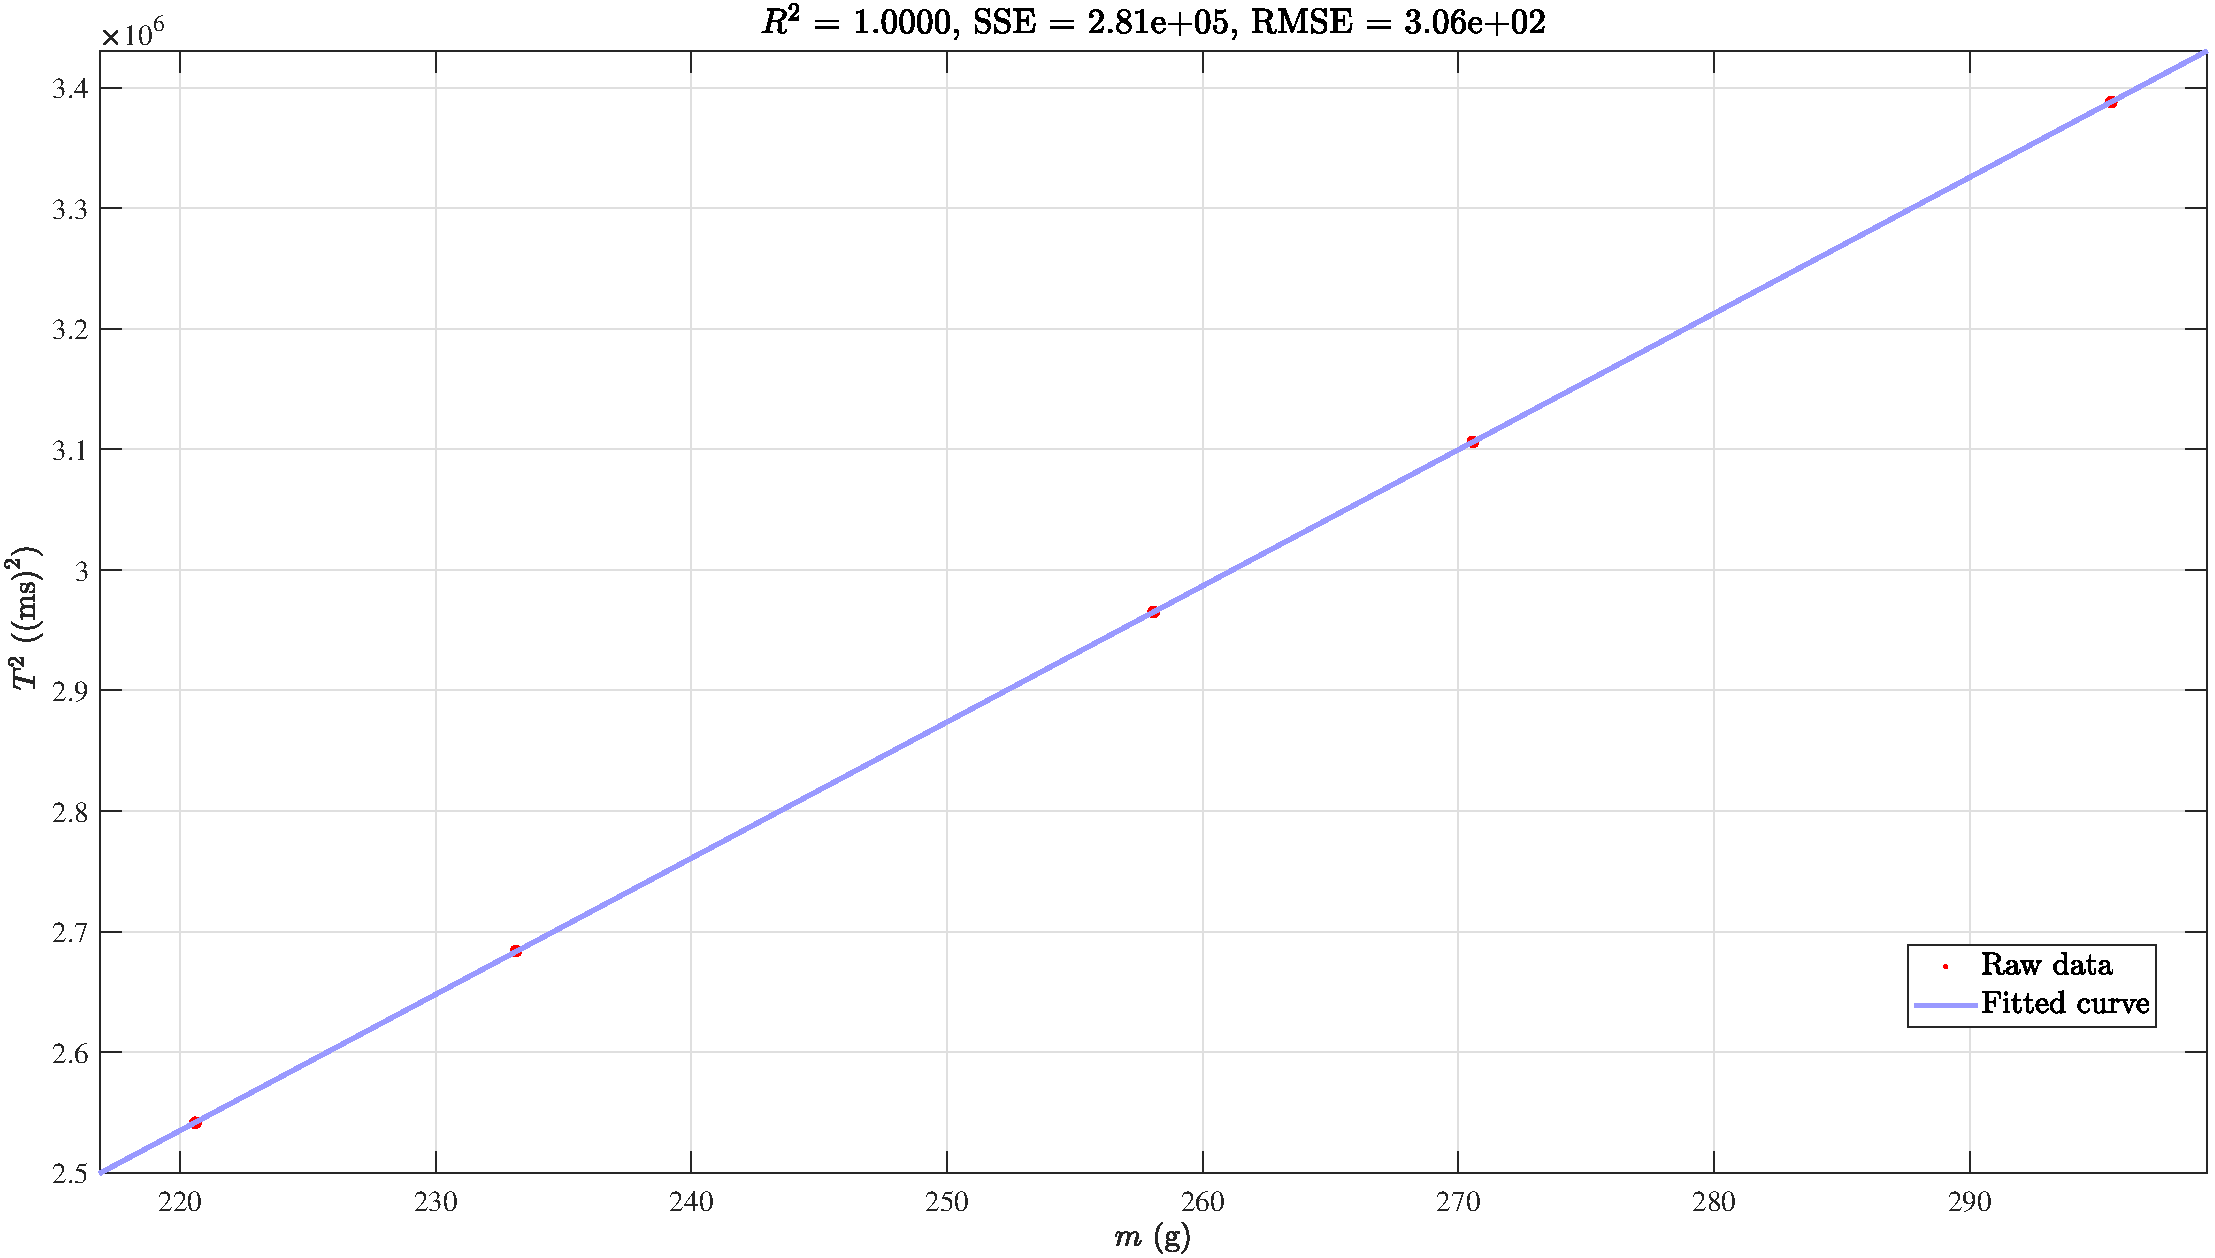
\includegraphics[width=0.9\columnwidth]{assets/表3.pdf}
    \caption{振子周期与质量的关系}
\end{figure}
    根据图像和相关拟合参数可知,拟合程度极好。图像斜率和截距分别为:
\begin{equation}
    a = 1.1296 \times 10^4 \ \mathrm{(ms)^2/g} = 11.296  \ \mathrm{s^2/kg},\quad 
    b = 4.9812 \times 10^4 \ \mathrm{(ms)^2} = 0.049812  \ \mathrm{s^2}
\end{equation}
    由实验原理部分,可知斜率为 $\frac{4{\pi ^2}}{k} $ ,截距为 $\frac{4{\pi ^2}m_0}{k}$ ,计算可得:
\begin{equation}
k = \frac{4\pi^2}{a} = 3.4949 \ \mathrm{N/m},\quad m_0 = \frac{bk}{4 \pi ^2} = 4.4097 \ \mathrm{g}
\end{equation}
也即弹簧的劲度系数为 $3.4949 \ \mathrm{N/m}$,弹簧的有效质量为 4.4097 g。

\subsection{研究速度与位移的关系}
    振子的振幅 $A$ 取40.0 cm,得到数据如下:
\begin{table}[H]\centering
    %\renewcommand{\arraystretch}{1.5} % 调整行间距为 1.5 倍
    %\setlength{\tabcolsep}{1.5mm} % 调整列间距
    \caption{速度与位移的关系}
    \label{速度与位移的关系}
\begin{tabular}{cccccccccc}\toprule
    位移 $x$ (cm) & 10 & 15 & 20 & 25 & 30  \\
    \midrule
    $v_1$ (cm/s) &148.37	&141.64	&132.98	&120.05	&100.30 \\
    $v_2$ (cm/s) &148.81	&142.25	&132.80	&121.31	&98.66  \\
    $v_3$ (cm/s) &148.59	&142.65	&132.62	&119.90	&100.00 \\
    $\overline{v}$ (cm/s) &148.59	&142.18	&132.80	&120.42	&99.65  \\
    \bottomrule
\end{tabular}
\end{table}
依据上面数据作线性拟合,并绘制图像:
\begin{equation}
y = -15.049 \, x + 2.3644
\end{equation}
\begin{figure}[H]\centering
    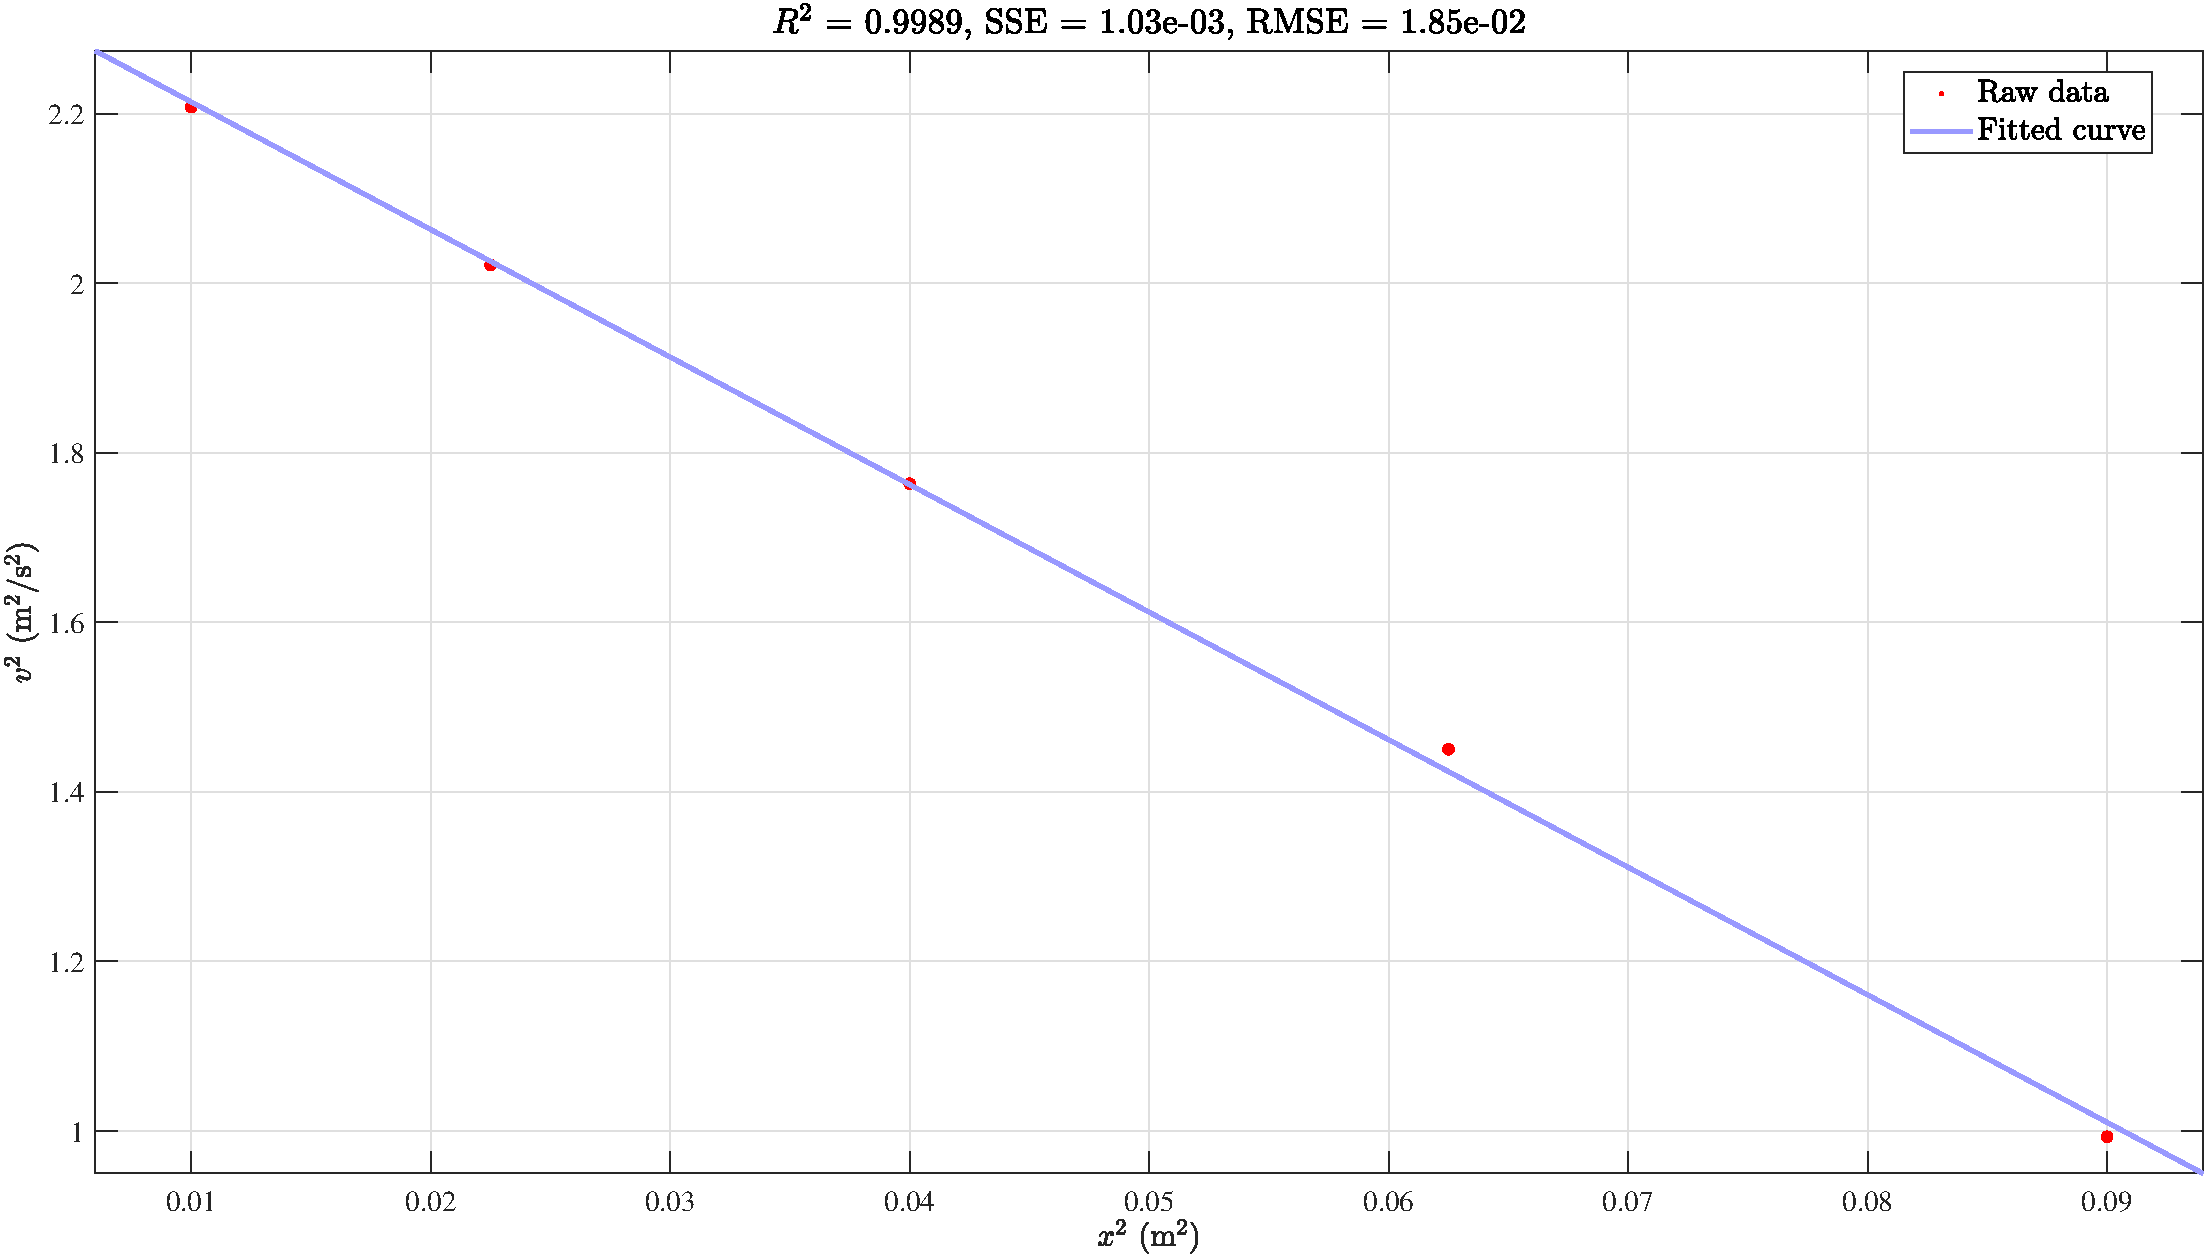
\includegraphics[width=0.9\columnwidth]{assets/表4.pdf}
    \caption{速度与位移的关系}
\end{figure}
    拟合直线斜率 $a = -1.5049$,截距 $b = 2.3644$,由原理部分公式可知:
\begin{equation}
\omega_0 = \sqrt{-a} = 3.8793 \ \mathrm{rad/s},\quad  T_0 = \frac{2\pi }{\omega_0}= 1619.67 \ \mathrm{ms}
\end{equation}
这与前面得到的 1593.76 ms 十分接近,在误差范围内可认为两者相等。


\subsection{研究机械能是否守恒}
    振子的振幅 $A$ 取40.0 cm,数据如下表所示,其中 $m = m_0 + m_1 = 225.01 \ \mathrm{g}$。
\begin{table}[H]\centering
    %\renewcommand{\arraystretch}{1.5} % 调整行间距为 1.5 倍
    %\setlength{\tabcolsep}{1.5mm} % 调整列间距
    \caption{不同位置的机械能情况}
    \label{不同位置的机械能情况}
\begin{tabular}{cccccccccc}\toprule
    $x$ (m) & 0.10 & 0.15 & 0.20 & 0.25 & 0.30  \\
    \midrule
    $v$ (m/s) &1.4859	&1.4218	&1.3280	&1.2042	&0.9965 \\
    $E_k$ (J)&0.2484	&0.2274	&0.1984	&0.1631	&0.1117 \\
    $E_p$ (J)&0.0175	&0.0393	&0.0699	&0.1092	&0.1573 \\
    $E$ (J)&0.2659	&0.2667	&0.2683	&0.2724	&0.2690 \\
    \bottomrule
\end{tabular}
\end{table}
    由机械能数据和下图可以认为,振动系统的机械能在振动过程中不变,与理论结果相符。
\begin{figure}[H]\centering
    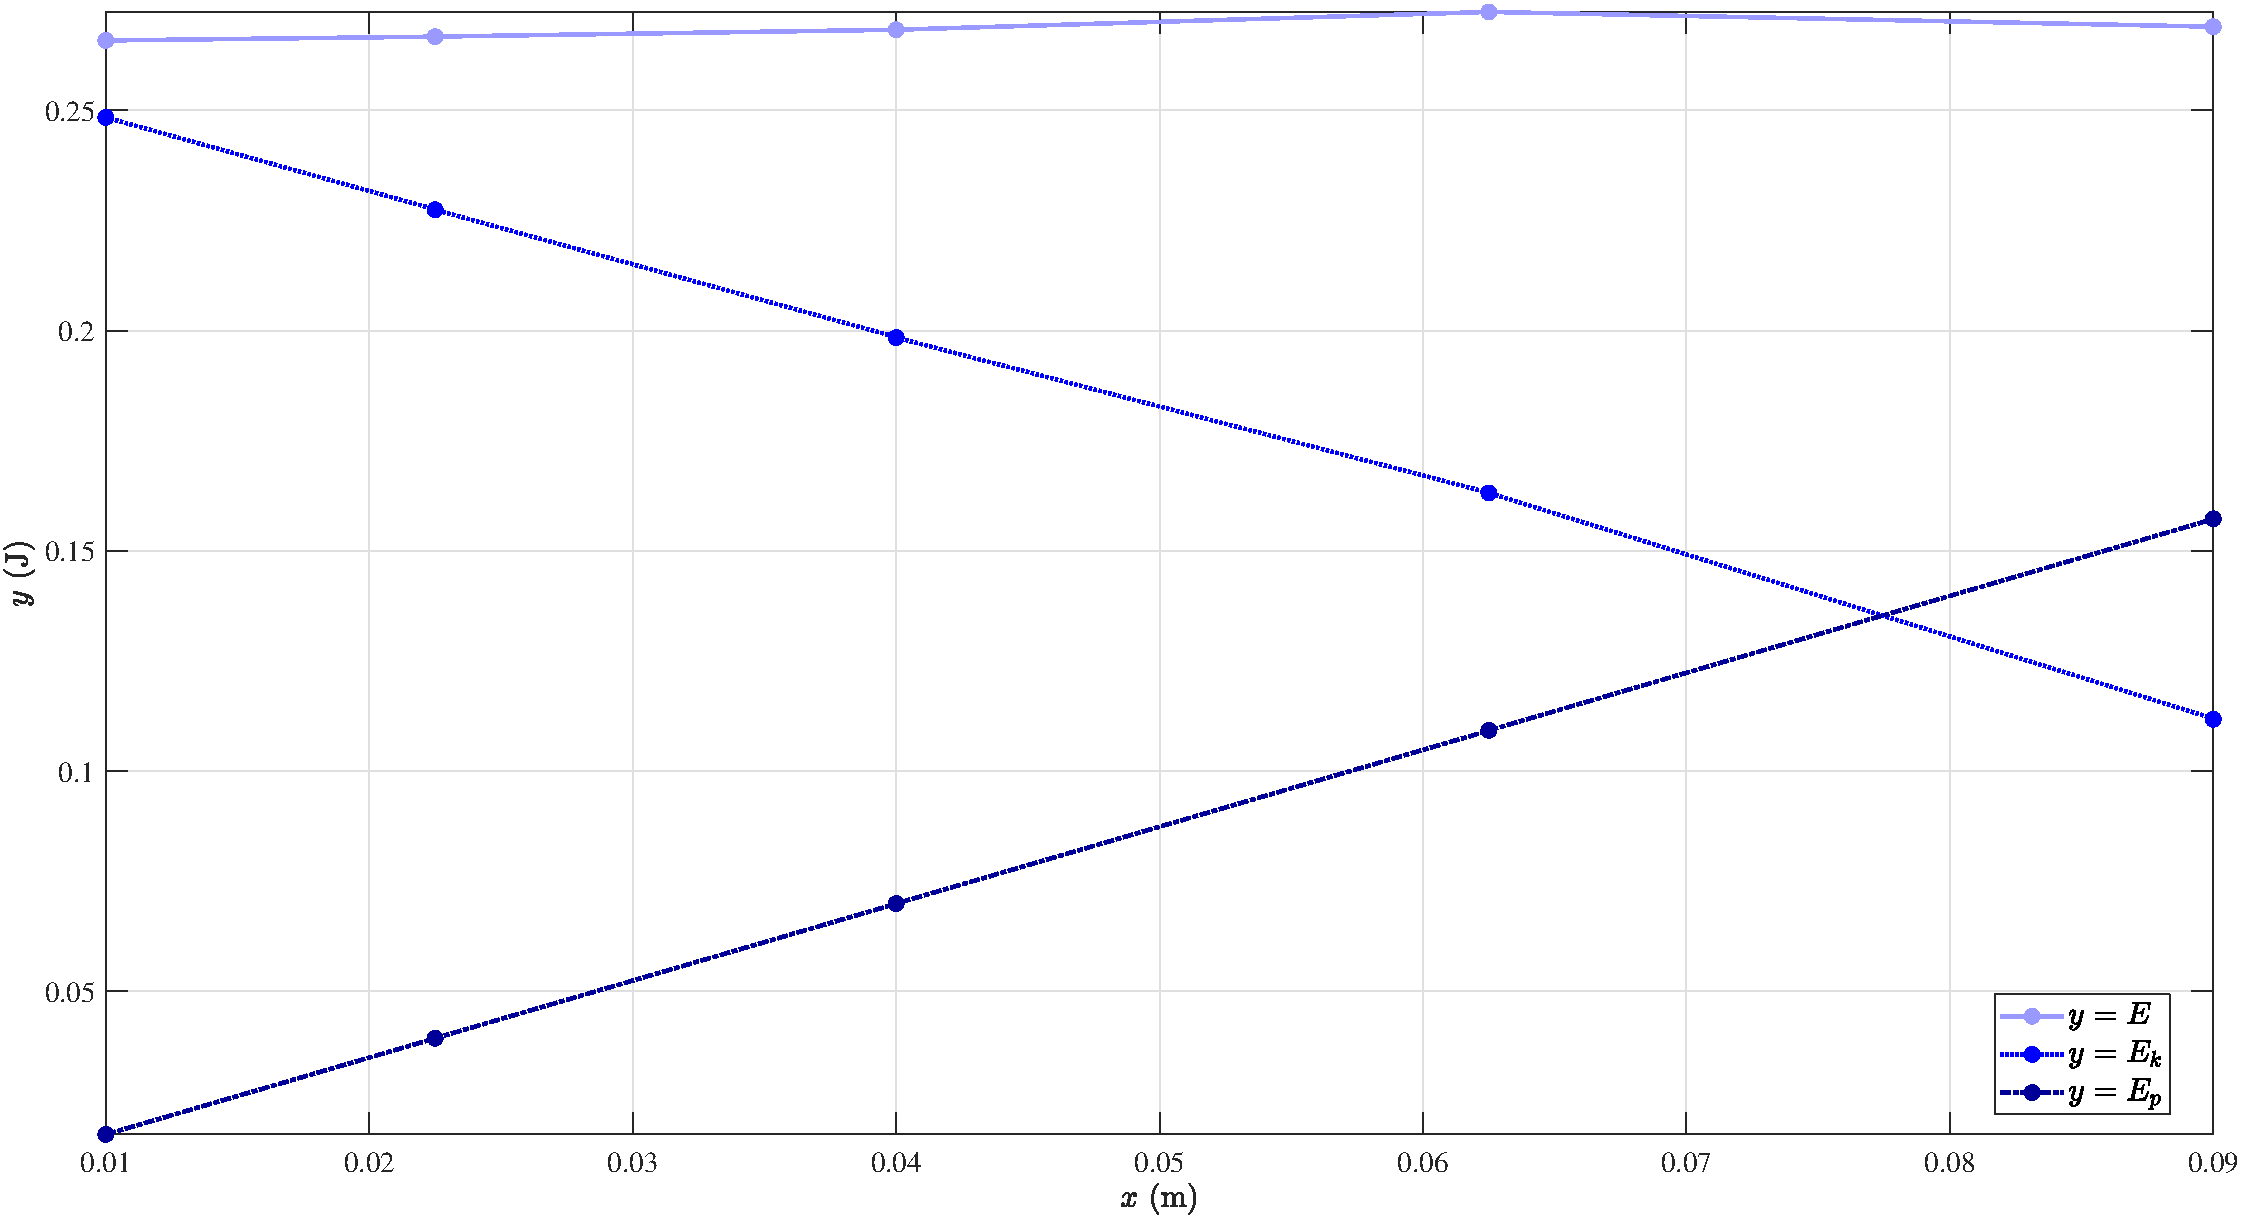
\includegraphics[width=0.9\columnwidth]{assets/5.pdf}
    \caption{不同位置的机械能情况}
\end{figure}

\subsection{改变振幅 $A$ ,测出相应的$v_{max}$,由${v_{max}}^2$-$A^2$图像求k}
不同振幅 $A$ 下的最大速度如下:
\begin{table}[H]\centering
    %\renewcommand{\arraystretch}{1.5} % 调整行间距为 1.5 倍
    %\setlength{\tabcolsep}{1.5mm} % 调整列间距
    \caption{振幅与最大速度的关系}
    \label{振幅与最大速度的关系}
\begin{tabular}{cccccccccc}\toprule
    $A$ (cm) & 10 & 15 & 20 & 25 &30 \\
    \midrule
    $v_{\max, 1}$ &38.90	&57.64	&76.92	&96.34	&115.47 \\
    $v_{\max, 2}$ &39.09	&57.67	&76.80	&96.33	&115.21 \\
    $v_{\max, 3}$ &39.21	&57.87	&77.04	&96.25	&115.20 \\
    $v_{\max}$ &39.07	&57.73	&76.92	&96.31	&115.29 \\
    \bottomrule
\end{tabular}
\end{table}
    依据上面数据作线性拟合,并绘制图像:
\begin{equation}
y = 14.796 \, x 
\end{equation}

\begin{figure}[H]\centering
    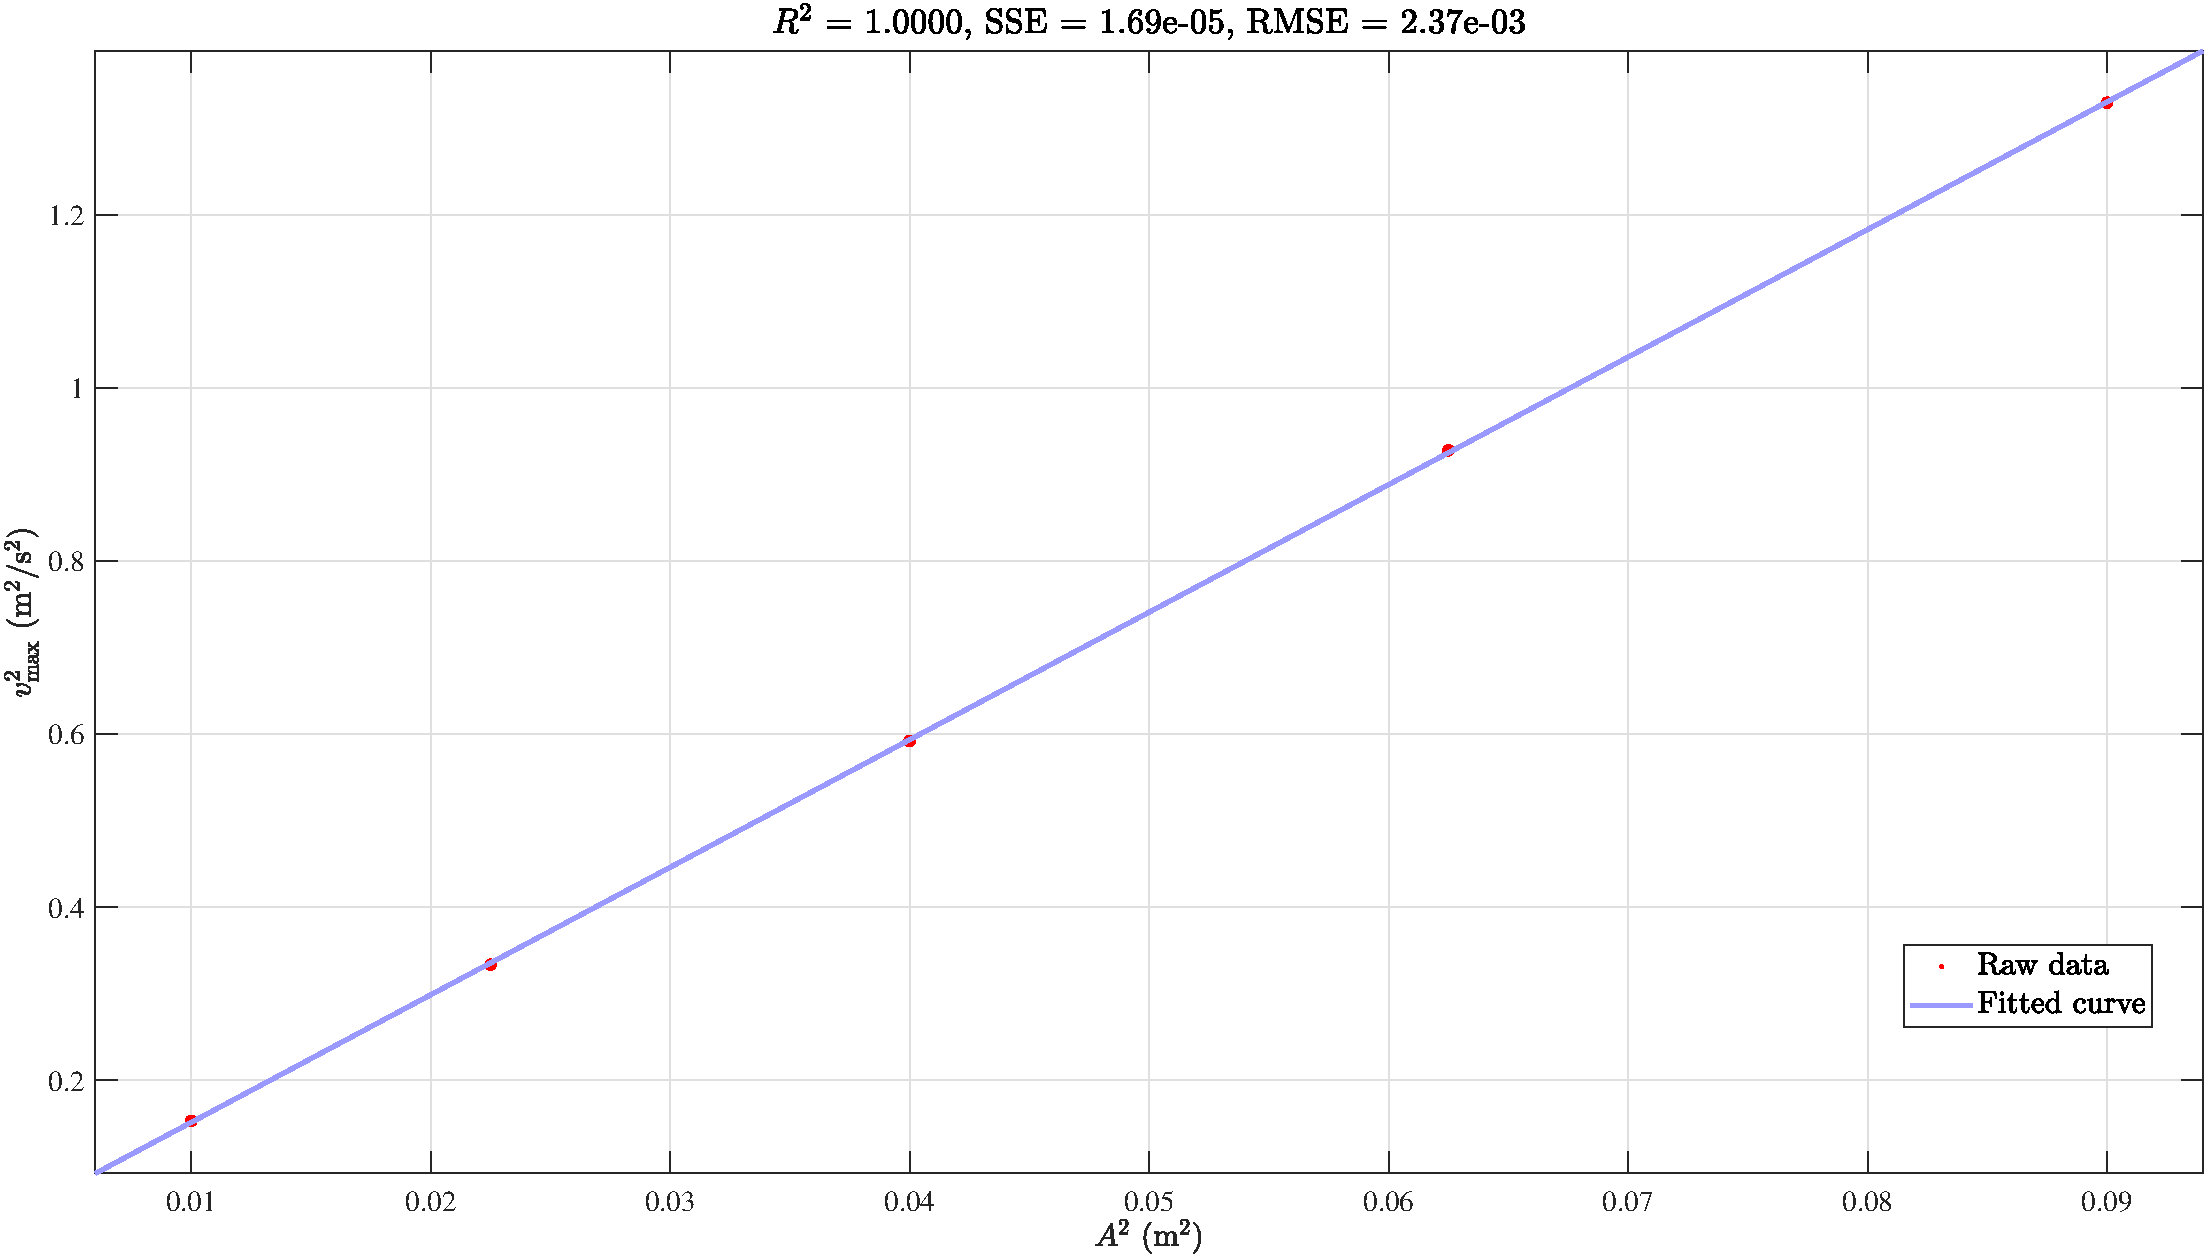
\includegraphics[width=0.9\columnwidth]{assets/6.pdf}
    \caption{振幅与最大速度的关系}
\end{figure}
拟合直线斜率 $a = 14.796$,于是:
\begin{equation}
\frac{1}{2}k A^2 = \frac{1}{2} m v_{\max}^2 \Longrightarrow 
k = ma = 3.3292 \ \mathrm{N/m}
\end{equation}
这与之前 $k = 3.4949 \ \mathrm{N/m}$ 的结果较为接近。

\subsection{其他相关参数}
\begin{enumerate}
\item 滑块质量 $m_1$ : 217.99 g
\item 条形挡光片质量: 2.61 g
\item U 型挡光片质量: 11.83 g
\end{enumerate}


\subsection{测定瞬时速度与不同U型挡光片通过光电门所用的时间(AP=50cm),计算平均速度}
此小节我们设定 Ap = 50 cm,并添加一块垫片以改变倾斜角度,得到数据如下:

\begin{table}[H]\centering
    %\renewcommand{\arraystretch}{1.5} % 调整行间距为 1.5 倍
    %\setlength{\tabcolsep}{1.5mm} % 调整列间距
    \caption{挡光片宽度与平均速度的关系(第一次)}
\begin{tabular}{cccccccccc}\toprule
    挡光片宽度 & $\Delta t_1$ (ms) & $\Delta t_2$ (ms) & $\Delta t_3$ (ms) & $\Delta t_4$ (ms) & $\Delta t_5$ (ms) & $\overline{\Delta t}$ (ms) & $\overline{v}$ (cm/s)  \\
    \midrule
    1 cm   &27.62	&27.53	&27.59	&27.79	&27.79	&27.66  & 0.361\\
    3  cm  &81.29	&81.70	&81.30	&81.70	&81.41	&81.48  & 0.368\\
    5  cm  &135.22	&135.17	&135.57	&135.61	&135.51	&135.42 & 0.369\\
    10  cm &262.67	&262.40	&263.47	&262.62	&263.20	&262.87 & 0.380\\
    \bottomrule
\end{tabular}
\end{table}
利用关系式 $\overline{v} = v_0 + \frac{1}{2}a \Delta t$,作线性拟合,可以得到:
\begin{figure}[H]\centering
    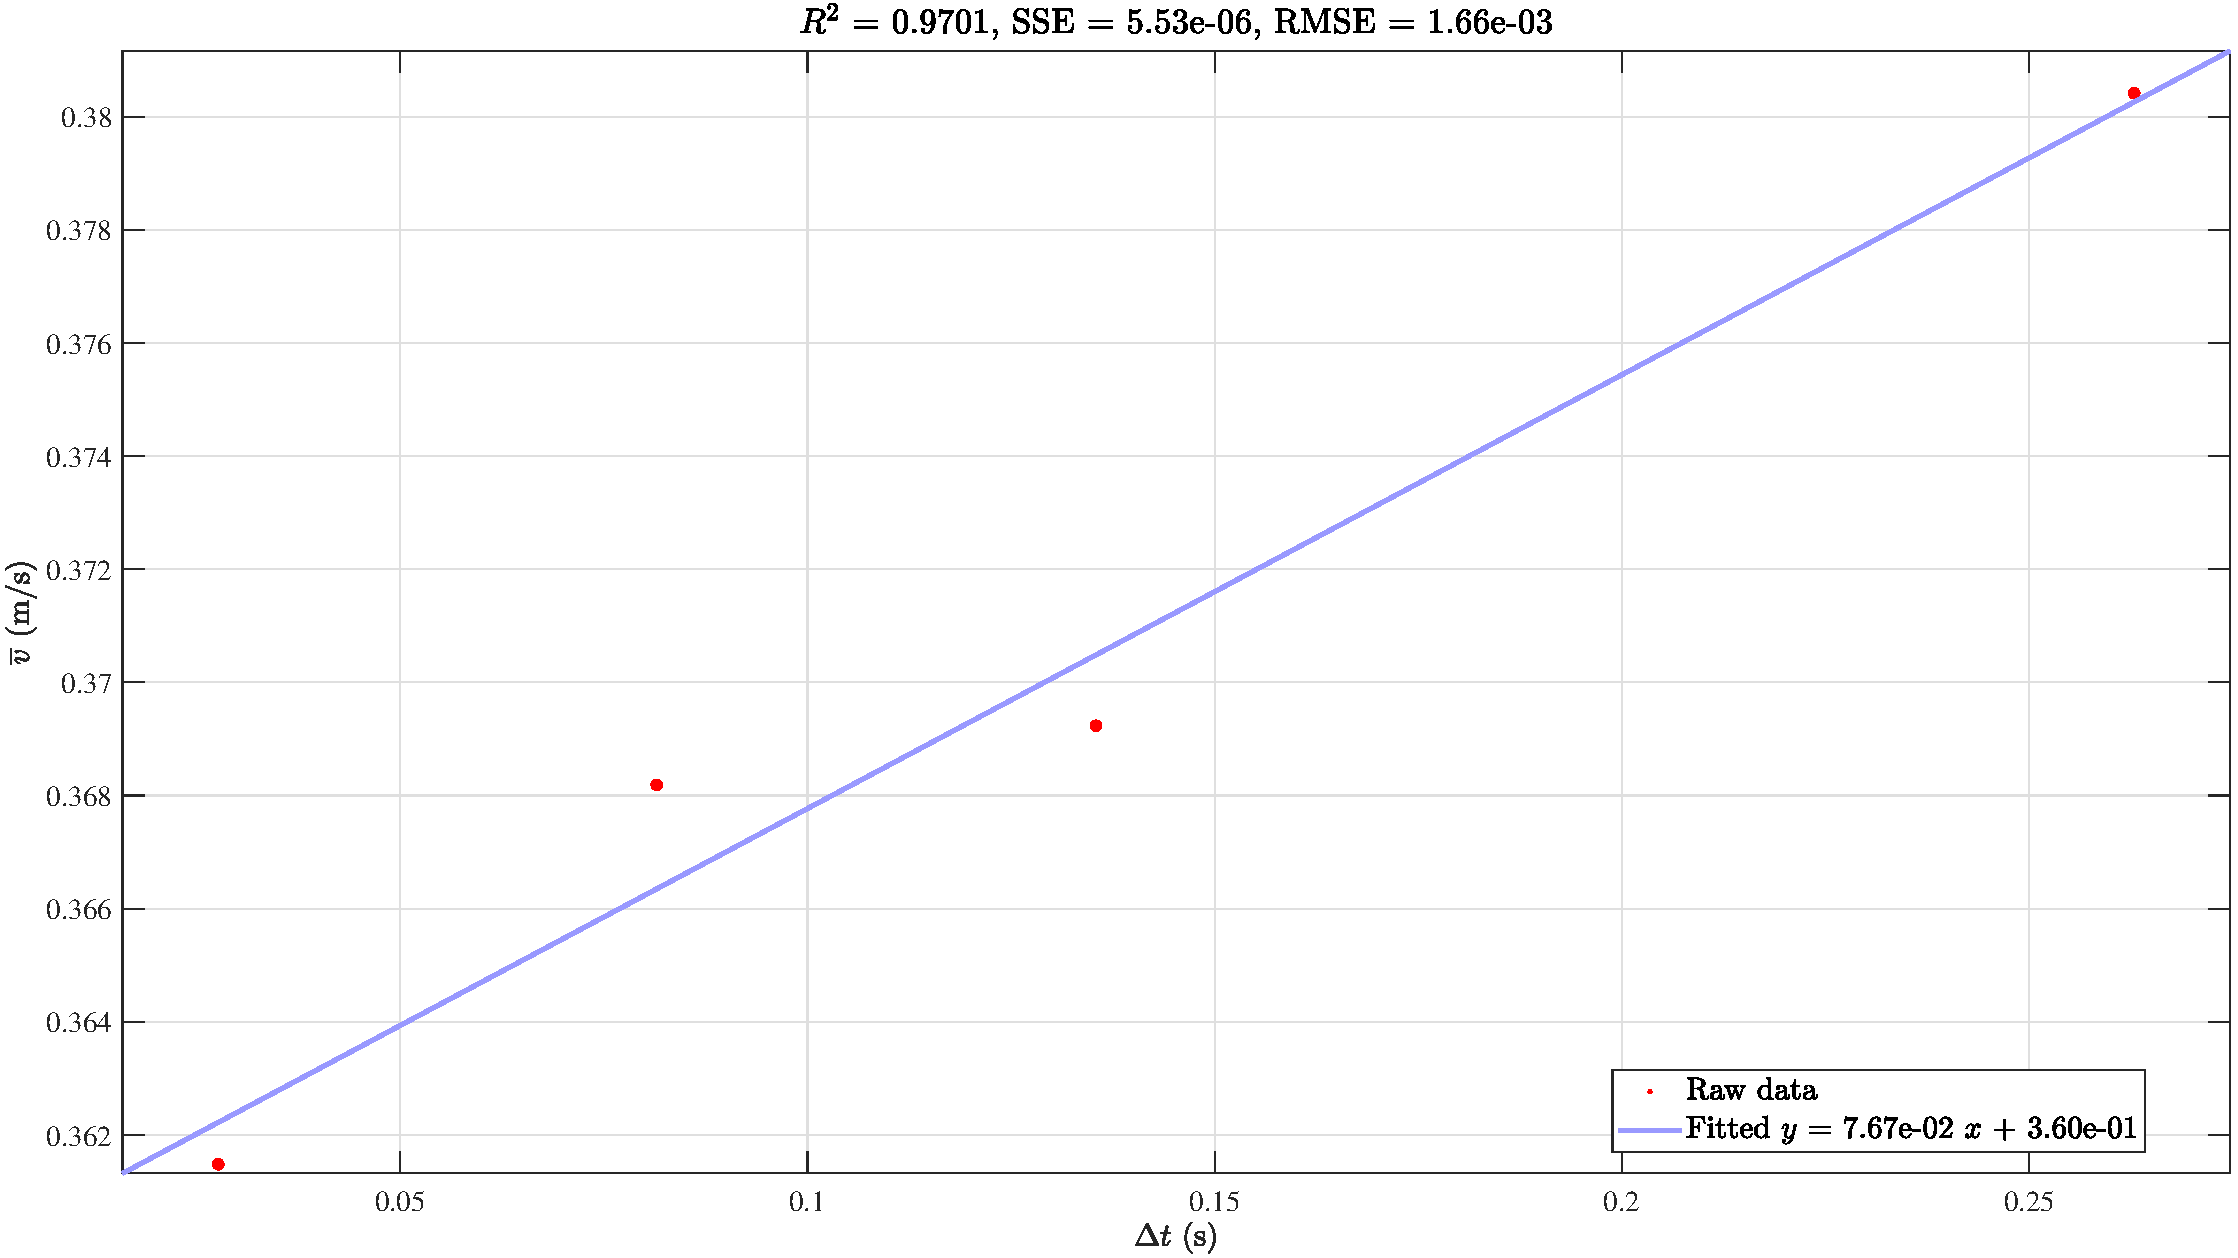
\includegraphics[width=0.9\columnwidth]{assets/8.pdf}
    \caption{挡光片宽度与平均速度的关系(第一次)}
\end{figure}
由截距可得 $v_0$ : 
\begin{equation}
v_0 = 0.360 \ \mathrm{m/s}
\end{equation}

\subsection{改变导轨倾角,测定瞬时速度与不同U型挡光片通过光电门所用的时间(AP=50cm),计算平均速度}
在上一小节的基础上,再添加一块垫片以增加倾斜角度,得到数据如下:
\begin{table}[H]\centering
    %\renewcommand{\arraystretch}{1.5} % 调整行间距为 1.5 倍
    %\setlength{\tabcolsep}{1.5mm} % 调整列间距
    \caption{挡光片宽度与平均速度的关系(第二次)}
\begin{tabular}{cccccccccc}\toprule
    挡光片宽度 & $\Delta t_1$ (ms) & $\Delta t_2$ (ms) & $\Delta t_3$ (ms) & $\Delta t_4$ (ms) & $\Delta t_5$ (ms) & $\overline{\Delta t}$ (ms) & $\overline{v}$ (m/s)  \\
    \midrule
    1 cm   &20.36	&20.30	&20.31	&20.38	&20.32	&20.33	&0.4918 \\
    3  cm  &60.01	&60.22	&60.20	&60.19	&60.15	&60.15	&0.4987 \\
    5  cm  &99.80	&100.05	&99.86	&100.10	&99.96	&99.95	&0.5002 \\
    10  cm &195.24	&195.10	&195.52	&195.70	&195.22	&195.36	&0.5119 \\
    \bottomrule
\end{tabular}
\end{table}
利用关系式 $\overline{v} = v_0 + \frac{1}{2}a \Delta t$,作线性拟合,可以得到:
\begin{figure}[H]\centering
    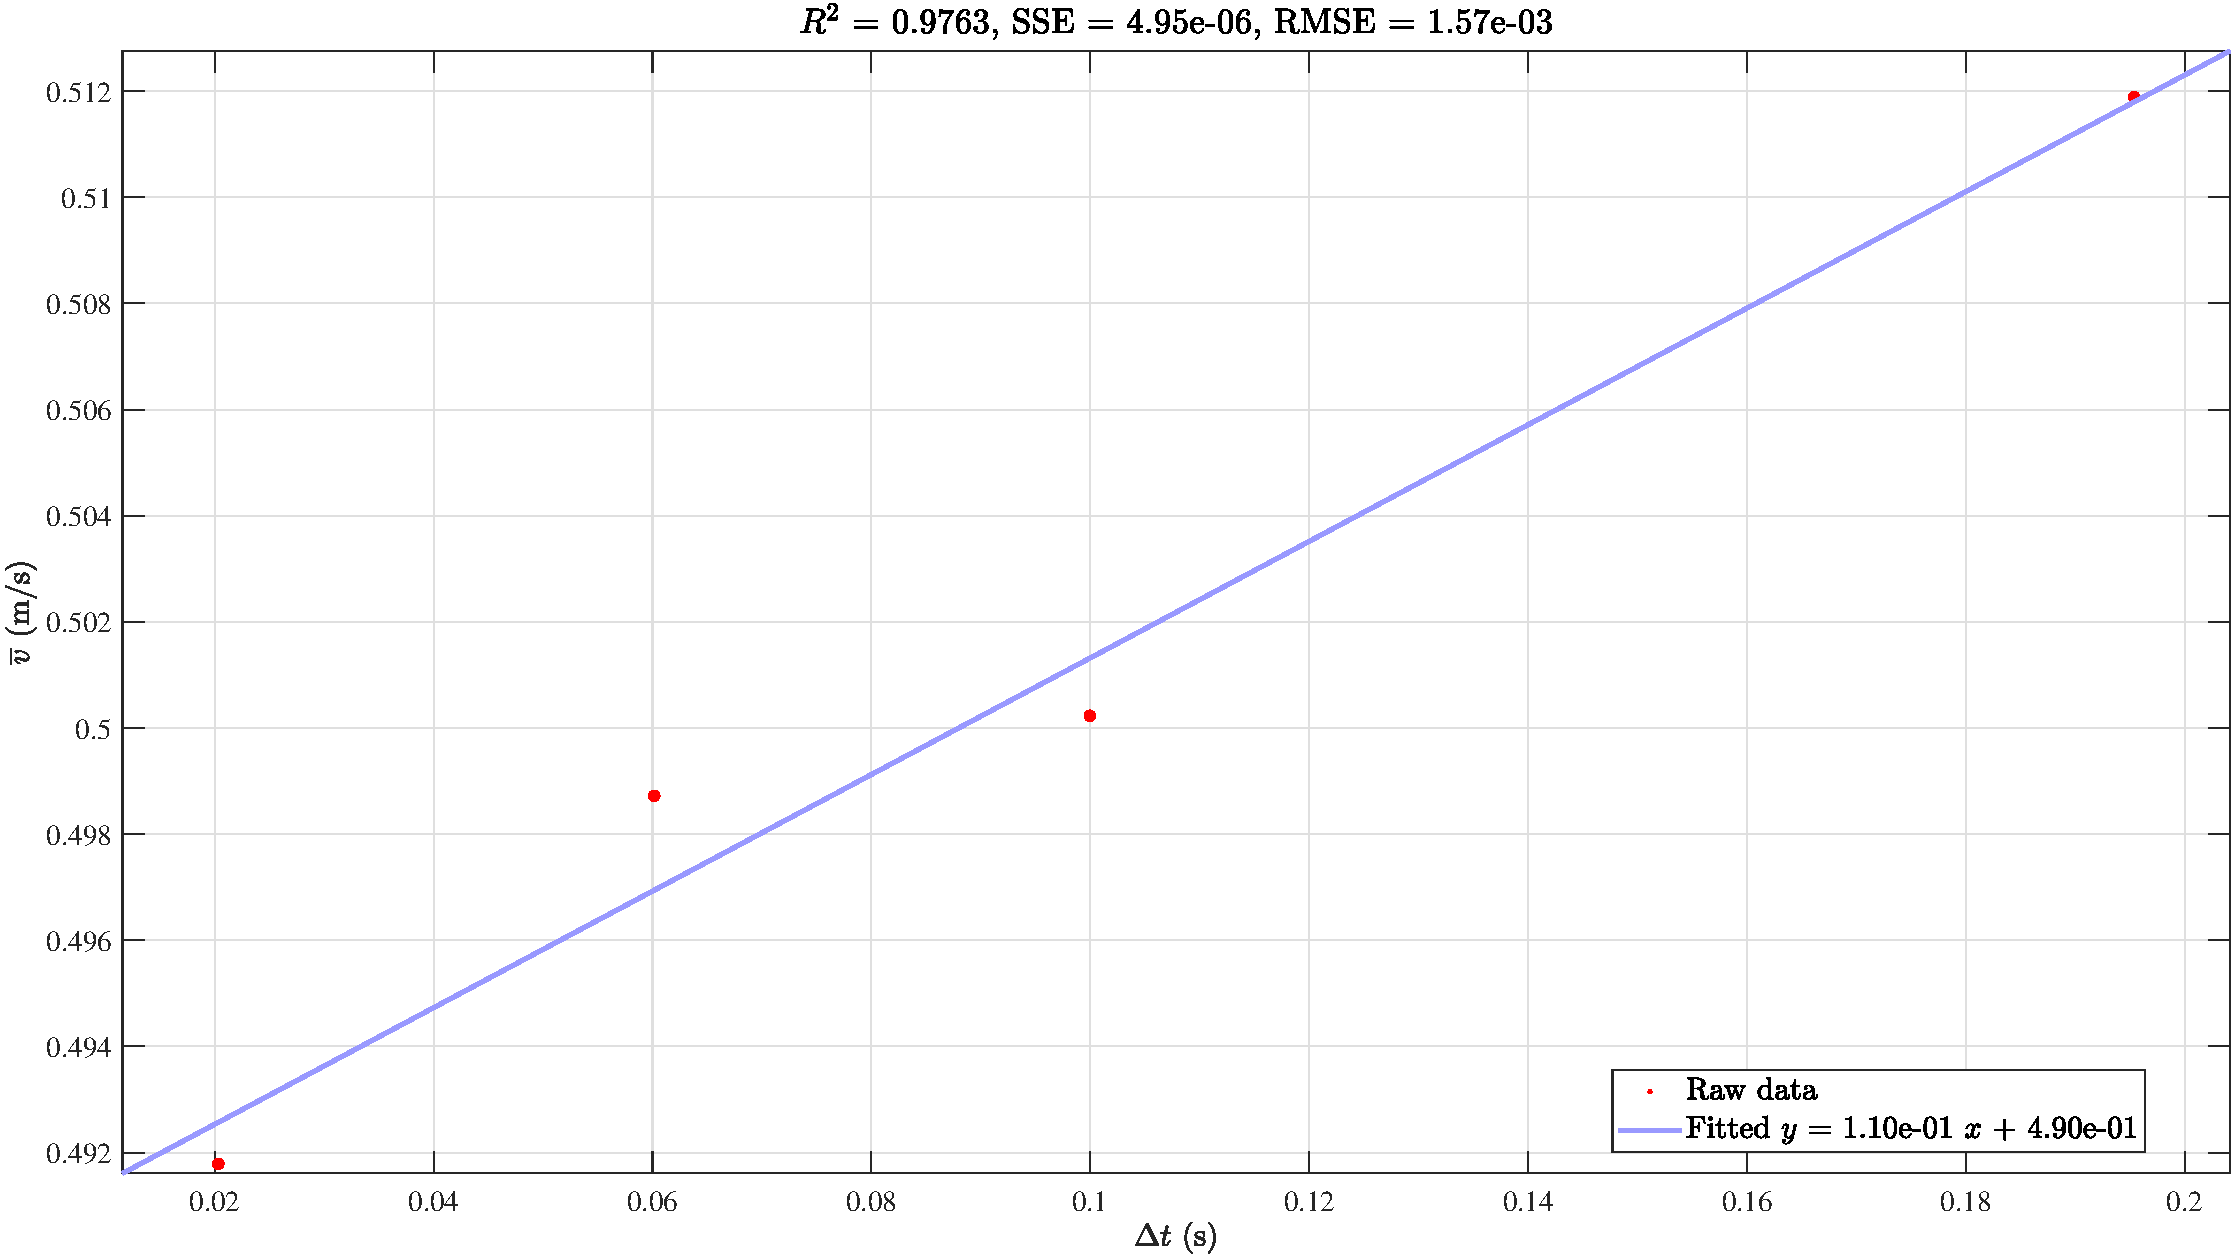
\includegraphics[width=0.9\columnwidth]{assets/9.pdf}
    \caption{挡光片宽度与平均速度的关系(第二次)}
\end{figure}
由截距可得 $v_0$ : 
\begin{equation}
v_0 = 0.490 \ \mathrm{m/s}
\end{equation}

\subsection{测定瞬时速度与不同U型挡光片通过光电门所用的时间(AP=60cm),计算平均速度}
在上一小节的基础上,保持倾斜角度不变,调整 AP 距离为 60 cm,得到数据如下:
\begin{table}[H]\centering
    %\renewcommand{\arraystretch}{1.5} % 调整行间距为 1.5 倍
    %\setlength{\tabcolsep}{1.5mm} % 调整列间距
    \caption{挡光片宽度与平均速度的关系(第三次)}
\begin{tabular}{cccccccccc}\toprule
    挡光片宽度 & $\Delta t_1$ (ms) & $\Delta t_2$ (ms) & $\Delta t_3$ (ms) & $\Delta t_4$ (ms) & $\Delta t_5$ (ms) & $\overline{\Delta t}$ (ms) & $\overline{v}$ (m/s)  \\
    \midrule
    1 cm   &18.54	&18.56	&18.56	&18.52	&18.53	&18.5420	&0.5393 \\
    3  cm  &54.85	&54.98	&54.82	&54.95	&54.96	&54.9120	&0.5463 \\
    5  cm  &91.47	&91.44	&91.18	&91.17	&91.40	&91.3320	&0.5475 \\
    10  cm &179.12 &179.54	&179.28	&179.52	&179.22	&179.3360	&0.5576 \\
    \bottomrule
\end{tabular}
\end{table}
利用关系式 $\overline{v} = v_0 + \frac{1}{2}a \Delta t$,作线性拟合,可以得到:
\begin{figure}[H]\centering
    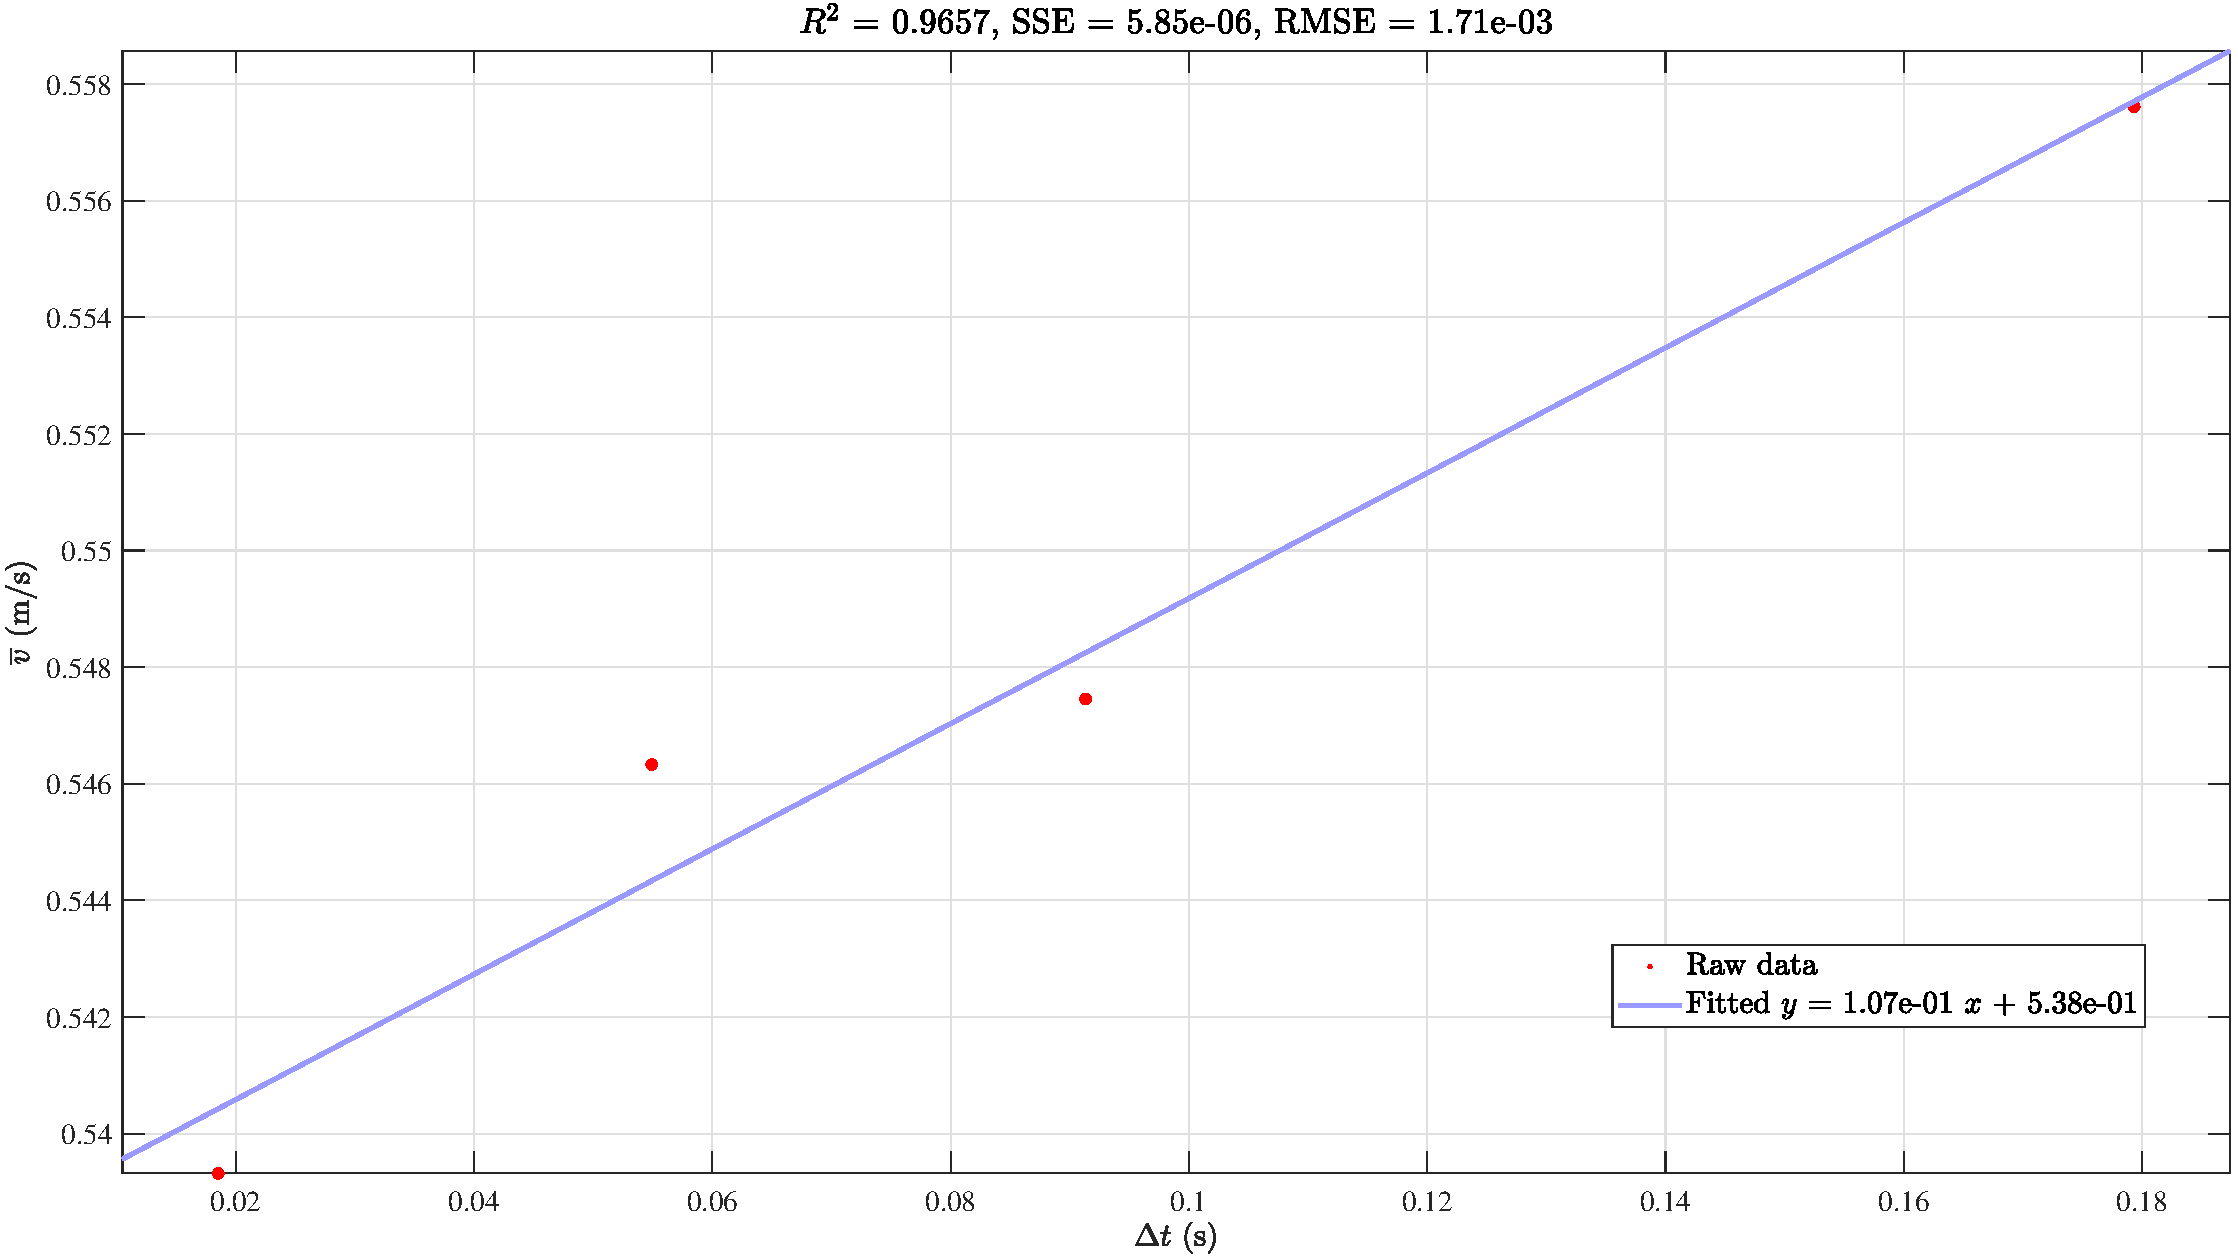
\includegraphics[width=0.9\columnwidth]{assets/10.pdf}
    \caption{挡光片宽度与平均速度的关系(第三次)}
\end{figure}
由截距可得 $v_0$ : 
\begin{equation}
v_0 = 0.538 \ \mathrm{m/s}
\end{equation}

\subsection{落球法测定液体在不同温度的粘度}
此小节的计算公式为:
\begin{equation}
v_0 = \frac{D}{\overline{t}},\quad \eta_{\text{expe}} = \frac{(\rho - \rho_0) g d^2}{18 v_0 \left(1 + \frac{2.4\, d}{D}\right)},\quad \text{error} = \frac{\eta_{\text{expe}}  - \eta_{\text{stan}}}{\eta_{\text{stan}} }\times 100\, \%
\end{equation}
其中 $\eta_{\text{expe}} $ 为实验测得的粘度系数,$\eta_{\text{stan}} $ 为标准值,$D = 0.2 \ \mathrm{m}$,$\rho = 7.8 \times 10^3 \ \mathrm{kg/m^3}$,$\rho_0 = 0.95 \times 10^3 \ \mathrm{kg/m^3}$,$d = 1.12 \ \mathrm{mm}$,$g = 9.8015 \ \mathrm{m/s^2}$,$\overline{t}$ 为此温度液滴下落的平均时间。所得数据及结果如下:
\begin{table}[H]\centering
    %\renewcommand{\arraystretch}{1.5} % 调整行间距为 1.5 倍
    %\setlength{\tabcolsep}{1.5mm} % 调整列间距
    \caption{落球法测定液体在不同温度的粘度}
    \label{落球法测定液体在不同温度的粘度}
\begin{tabular}{ccccccccccccccc}\toprule
    温度 (\textcelsius) & $t_1$ (s) & $t_2$ (s) & $t_3$ (s) & $t_4$ (s) & $t_5$ (s) & $\overline{t}$ (s) & $v_0$ (m/s) & $\eta_{\text{expe}}$ (Pa$\cdot$s) & $\eta_{\text{stan}}$ (Pa$\cdot$s)  & error (\%)\\
    \midrule
    25 &25.10	&25.53	&25.50	&25.31	&25.55	&25.40	&0.0079	&0.5863	&0.6210 &-5.5881   \\
    30 &19.52	&19.47	&19.44	&19.47	&19.20	&19.42	&0.0103	&0.4483	&0.4510 &-0.5989   \\
    35 &14.87	&14.06	&14.31	&14.08	&14.16	&14.30	&0.0140	&0.3300	&0.3120 &5.7695    \\
    40 &10.41	&10.03	&10.09	&10.10	&10.00	&10.13	&0.0198	&0.2338	&0.2310 &1.1916    \\
    45 &7.44	&7.41	&7.31	&7.28	&7.34	&7.36	&0.0272	&0.1698	&0.1720 &-1.2739   \\
    50 &5.60	&5.50	&5.50	&5.50	&5.47	&5.51	&0.0363	&0.1273	&0.1260 &1.0217    \\
    55 &4.13	&4.18	&4.20	&4.19	&4.18	&4.18	&0.0479	&0.0964	&0.0980 &-1.6322   \\
    \bottomrule
\end{tabular}
\end{table}
如图所示:
\begin{figure}[H]\centering
    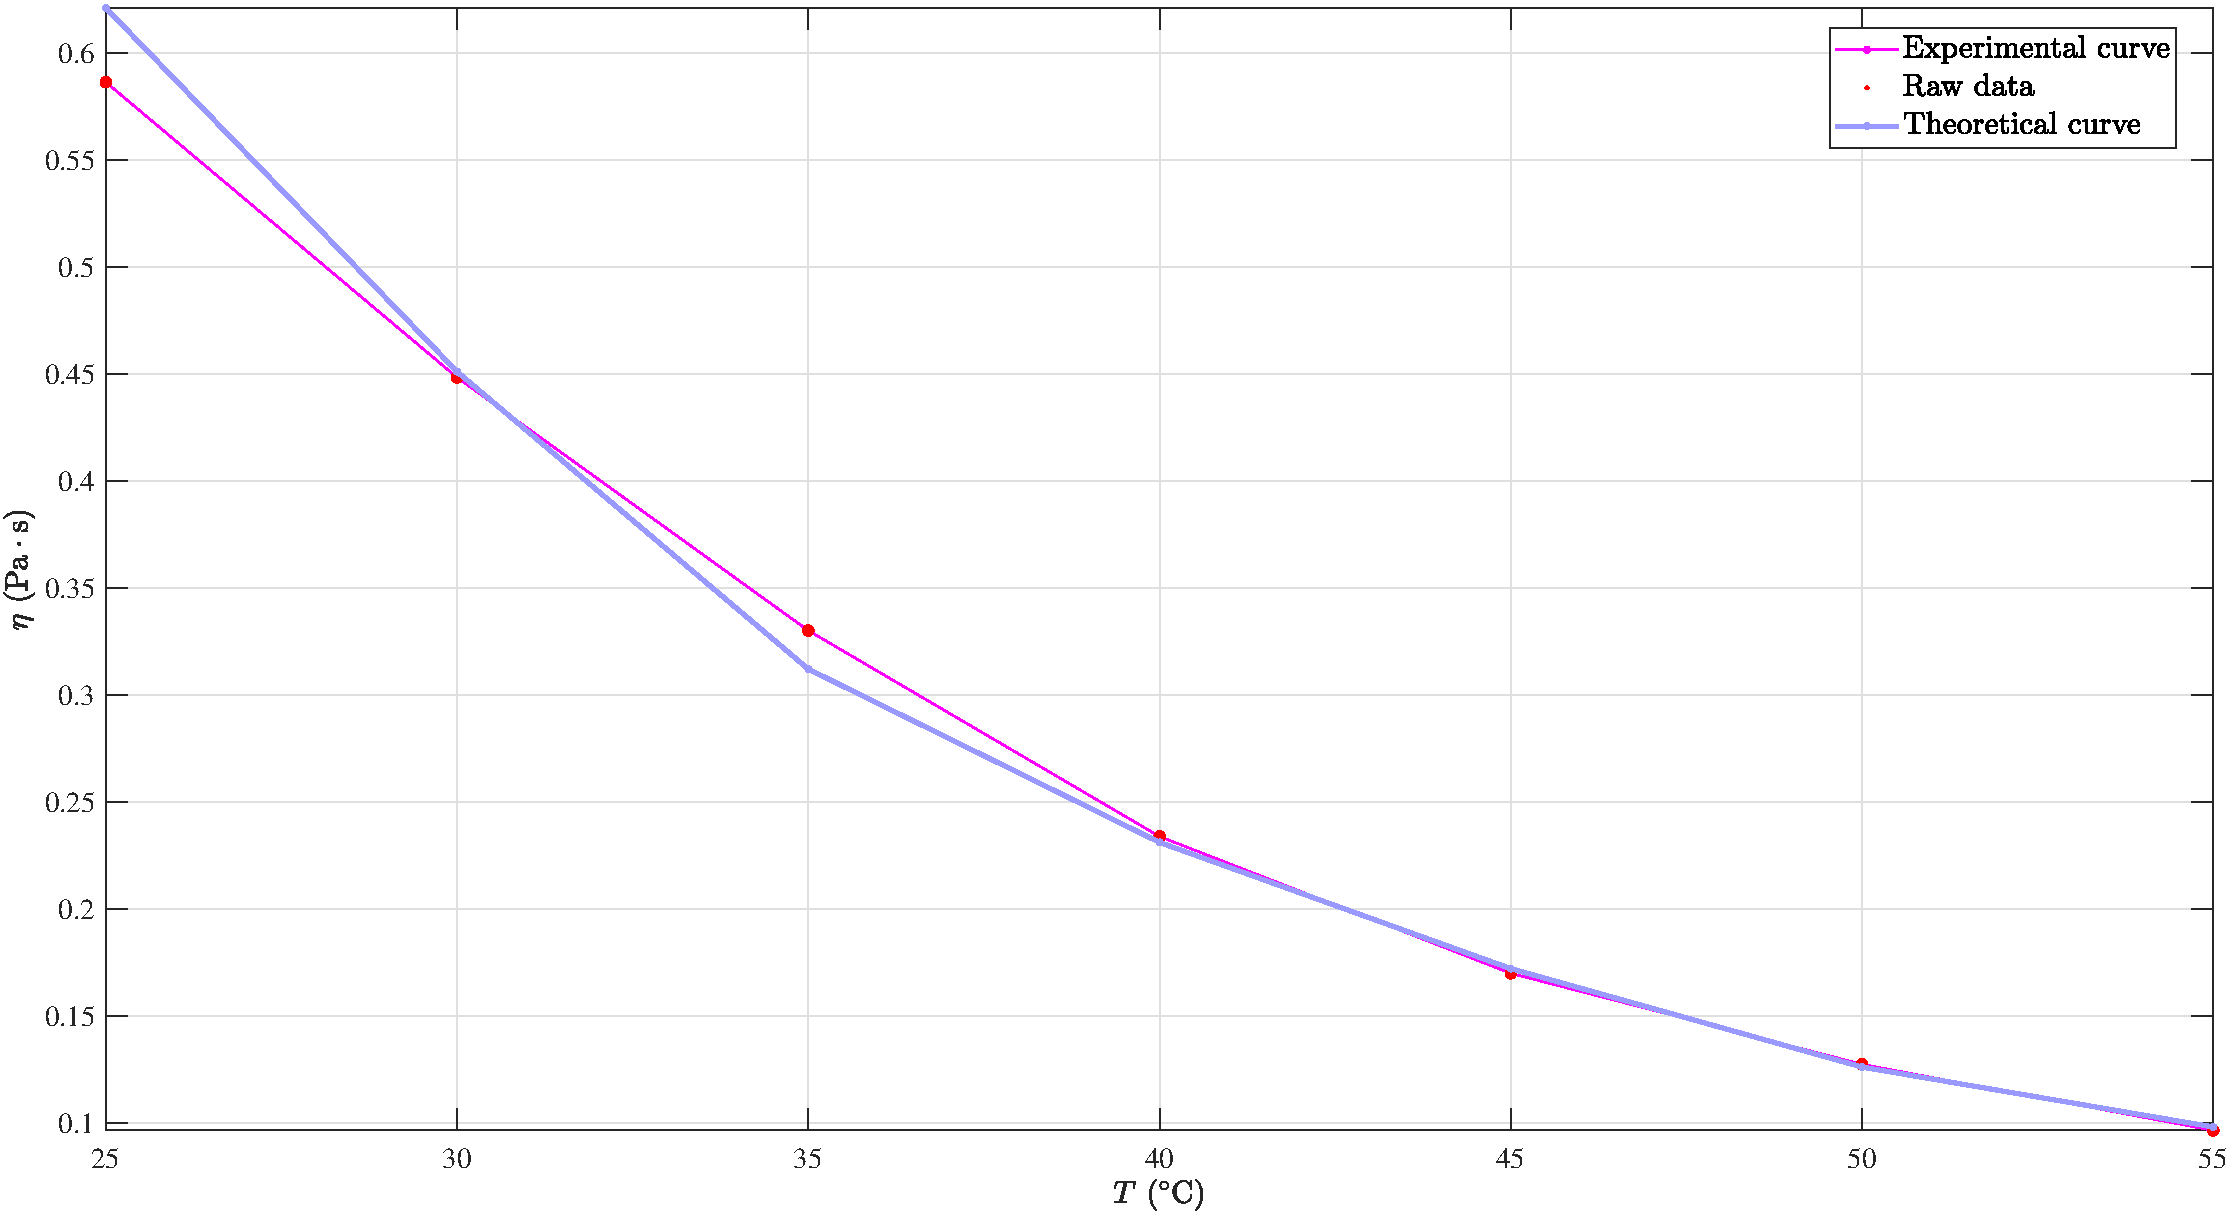
\includegraphics[width=0.9\columnwidth]{assets/eta.pdf}
    \caption{液体在不同温度下的粘度}
\end{figure}

\section{思考题}

\subsection*{6.1 \ \  仔细观察,可以发现滑块的振幅是不断减小的,那么为什么还可以认为滑块是做简谐振动?实验中应如何尽量保证滑块做简谐振动?}
振幅不断减小是由于存在阻尼,而我们之所以仍认为滑块作简谐振动,是因为气垫导轨摩擦较小,对实验结果的影响不是很大,事实上实际运动是欠阻尼简谐振动。在不考虑耗散的情况下,可近似认为是简谐运动。

实验中,我们使用气垫导轨以消除滑动摩擦;保证气垫导轨的水平;先打开气垫导轨再放置滑块;用光电门和数字毫秒计测量周期和速度,这些都可以尽量保证其做简谐振动。

\subsection*{6.2 \ \  试说明弹簧的等效质量的物理意义,如不考虑弹簧的等效质量,对实验结果有什么影响?}

因为实际上,弹簧本身的质量不可忽略,而质量的存在会导致弹簧内产生驻波,因而,严格来说,此时运动已经不满足简谐振动方程。为使简谐振动的原理尽可能被满足,亦即减小误差,我们考虑将这部分造成的影响用“等效质量”的概念代替:如果忽略高阶小量的话,那么就可以认为振动时仍保持质量线性分布,并且弹簧质量远小于滑块质量,由此大致上便解决了问题,更方便分析、计算。

如不考虑弹簧的等效质量,则可能会出现能量不守恒等情况,总机械能偏小,造成误差。

\subsection*{6.3 \ \  测量周期时,光电门是否必须在平衡位置上?如不在平衡位置会产生什么不同的效果?}
理论上并不需要,这对我们的测量结果并没有影响。

不过,在实际操作的过程中,由于存在能量耗散,导致振幅减小,如果不在平衡位置将会不便测量,造成较大的误差。此外,不在平衡位置导致每次测量的时候不处于周期的同一位置,这也势必会很不方便测量。

\subsection*{6.4 \ \  气垫导轨如果不水平,是否能进行该实验?}
理论上来说,如果只是为了观察简谐运动的性质,那么其实是不需要调平的,而且甚至于说,在忽略弹簧重力的情况下,机械能守恒的验证也并不会受到影响。只不过此时的公式会更加繁杂,需要考虑修正,这是不够便利的。

\subsection*{6.5 \ \  使用平板形挡光片和两个光电门,如何测量滑块通过倾斜气轨上某一点的瞬时速度?}

目标还是测量“瞬时”速度,因而实验思路大致上其实是不变的,仍然是通过改变距离,进而改变$\Delta s$,并测得其相应的$\Delta t$,通过线性拟合得到类似的结论。

\subsection*{6.6 \ \ 气垫导轨如果不水平,对瞬时速度的测定有什么影响?}

并不影响。事实上,测定瞬时速度的实验,还会要求我们的气垫导轨不水平。

\subsection*{6.7 \ \ 每次测量滑块和 U 型挡光片总质量不同是否对瞬时速度测定有影响?}
理论上应该是没有的,因为加速度与具体的质量值有关,进而,速度值也与具体的质量值无关。不过,不排除总质量不同导致表面积不同、进而导致阻力不同等情况造成的影响。




\section{实验总结与心得体会}


此次“气垫导轨”实验共分为两个部分,分别是弹簧振子的简谐运动和倾斜导轨上滑块的瞬时速度,实验步骤均比较简单。实验的一个重要思想线性拟合,以及“将复杂的乘除依赖关系转化为变量间的线性关系”,令我印象深刻;另一重点是数据的计算与拟合,在处理的过程中,我也学到很多。实验总体上是成功的,每个小节的实验都大致符合理论,实验数据和图像也具有较强的说服力。

特别地,在本次实验,我利用了 Matlab 软件对实验数据作进一步的处理和分析,包括换算、拟合、可视化等,相比于常规数据处理和画图方法,这大大提高了数据分析处理的速度的准确度,也提高了作图的美观性。在今后的实验和研究工作中,我还会继续深入学习和应用类似地计算软件,增强自己的科学计算能力。科研不是考试,我们应该充分利用好自己能接触到的资源,合理使用工具,更高效地发展自身。

另外,这次实验让我感受到,实验“结束”并不意味着实验就已经完成,事实上这仅是数据测量的结束。在课后,我们还需要重新整理实验原理和过程,换算、分析、拟合实验数据,作出合适的数据图,解释可能存在的误差等。在根据已有数据求所需结果时,如何才能最大程度地利用已有数据,同时又尽可能地降低二次误差。上面这些内容都需要体现在最终的实验报告中,一点点累加起来,着实花费了我很多精力。

但最后回过头来,我认为一切都是值得的。当处理完毕的结果有力地验证了理论值时,当实验数据图像与理论较好地契合时,心中便迸发出无尽的喜悦,也深深感受到物理“理论与实验结合”的魅力\footnote{本次实验的预习报告是撰写实验报告的前半部分,内容是重复的,因此不再给出;实验数据记录表和 Matlab 源码附在附录中}。





\newpage
\subsection*{附录 A\hspace*{20pt} 原始数据记录表}
\addcontentsline{toc}{section}{附录 A\hspace*{6pt} 原始数据记录表} 
\thispagestyle{fancy} 

\begin{figure}[H]\centering
    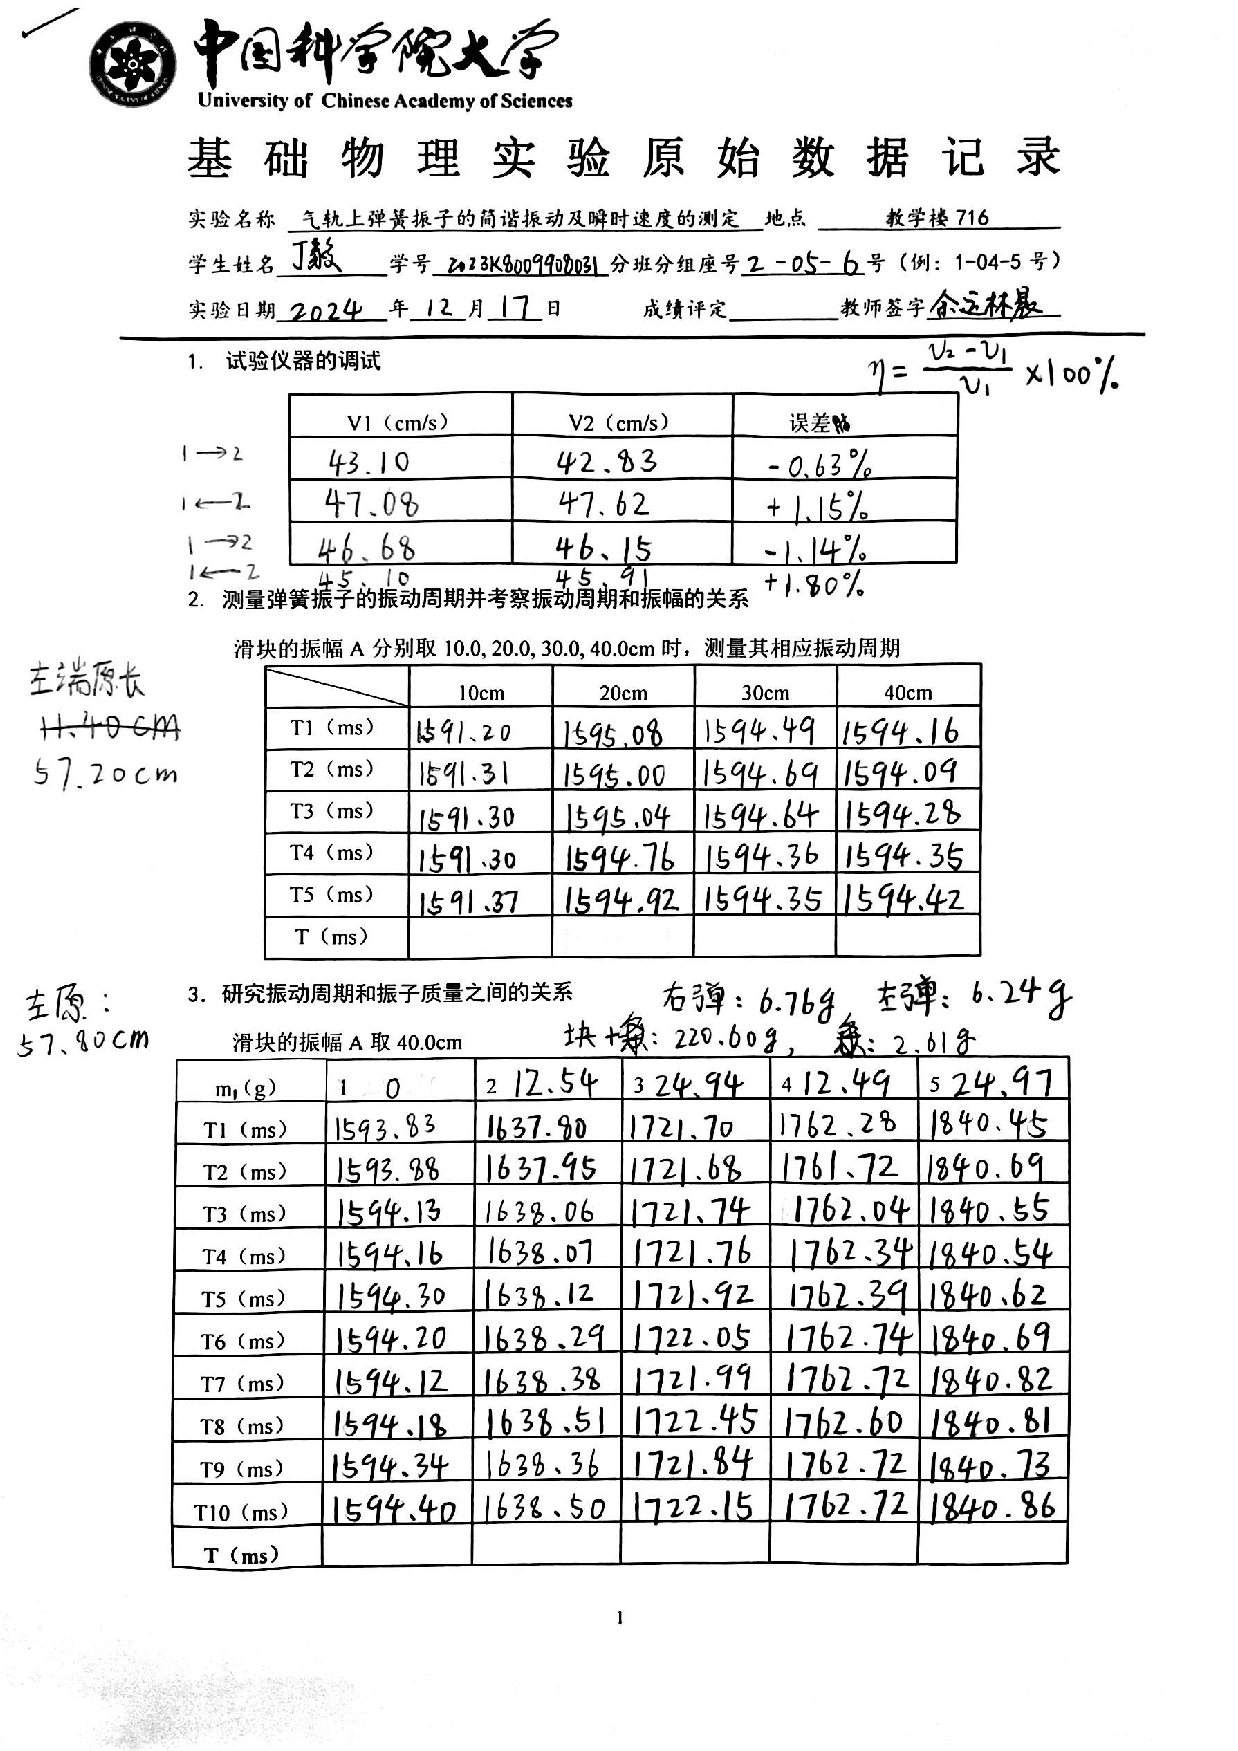
\includepdf[pages=1, width=480pt]{pdf/原始数据-2-05组-丁毅-气垫导轨-2024.12.18-余运林晨.pdf}
\end{figure}
\includepdf[pages={2,3}]{pdf/原始数据-2-05组-丁毅-气垫导轨-2024.12.18-余运林晨.pdf}

\subsection*{附录 B\hspace*{20pt} Matlab 源码}
\addcontentsline{toc}{section}{附录 B\hspace*{6pt} Matlab 源码} 
\thispagestyle{fancy} 
\lstinputlisting{d:/a_RemoteRepo/GH.MatlabCodes/本科课程代码/基础物理实验/Ex_5/Ex_05_mflie.m}





\end{document}

% VScode 常用快捷键:

% F2:                       变量重命名
% Ctrl + Enter:             行中换行
% Alt + up/down:            上下移行
% 鼠标中键 + 移动:           快速多光标
% Shift + Alt + up/down:    上下复制
% Ctrl + left/right:        左右跳单词
% Ctrl + Backspace/Delete:  左右删单词    
% Shift + Delete:           删除此行
% Ctrl + J:                 打开 VScode 下栏(输出栏)
% Ctrl + B:                 打开 VScode 左栏(目录栏)
% Ctrl + `:                 打开 VScode 终端栏
% Ctrl + 0:                 定位文件
% Ctrl + Tab:               切换已打开的文件(切标签)
% Ctrl + Shift + P:         打开全局命令(设置)

% Latex 常用快捷键:

% Ctrl + Alt + J:           由代码定位到PDF


